% Options for packages loaded elsewhere
\PassOptionsToPackage{unicode}{hyperref}
\PassOptionsToPackage{hyphens}{url}
%
\documentclass[
  11pt,
]{article}
\usepackage{amsmath,amssymb}
\usepackage{iftex}
\ifPDFTeX
  \usepackage[T1]{fontenc}
  \usepackage[utf8]{inputenc}
  \usepackage{textcomp} % provide euro and other symbols
\else % if luatex or xetex
  \usepackage{unicode-math} % this also loads fontspec
  \defaultfontfeatures{Scale=MatchLowercase}
  \defaultfontfeatures[\rmfamily]{Ligatures=TeX,Scale=1}
\fi
\usepackage{lmodern}
\ifPDFTeX\else
  % xetex/luatex font selection
\fi
% Use upquote if available, for straight quotes in verbatim environments
\IfFileExists{upquote.sty}{\usepackage{upquote}}{}
\IfFileExists{microtype.sty}{% use microtype if available
  \usepackage[]{microtype}
  \UseMicrotypeSet[protrusion]{basicmath} % disable protrusion for tt fonts
}{}
\makeatletter
\@ifundefined{KOMAClassName}{% if non-KOMA class
  \IfFileExists{parskip.sty}{%
    \usepackage{parskip}
  }{% else
    \setlength{\parindent}{0pt}
    \setlength{\parskip}{6pt plus 2pt minus 1pt}}
}{% if KOMA class
  \KOMAoptions{parskip=half}}
\makeatother
\usepackage{xcolor}
\usepackage[margin=1in]{geometry}
\usepackage{color}
\usepackage{fancyvrb}
\newcommand{\VerbBar}{|}
\newcommand{\VERB}{\Verb[commandchars=\\\{\}]}
\DefineVerbatimEnvironment{Highlighting}{Verbatim}{commandchars=\\\{\}}
% Add ',fontsize=\small' for more characters per line
\usepackage{framed}
\definecolor{shadecolor}{RGB}{248,248,248}
\newenvironment{Shaded}{\begin{snugshade}}{\end{snugshade}}
\newcommand{\AlertTok}[1]{\textcolor[rgb]{0.94,0.16,0.16}{#1}}
\newcommand{\AnnotationTok}[1]{\textcolor[rgb]{0.56,0.35,0.01}{\textbf{\textit{#1}}}}
\newcommand{\AttributeTok}[1]{\textcolor[rgb]{0.13,0.29,0.53}{#1}}
\newcommand{\BaseNTok}[1]{\textcolor[rgb]{0.00,0.00,0.81}{#1}}
\newcommand{\BuiltInTok}[1]{#1}
\newcommand{\CharTok}[1]{\textcolor[rgb]{0.31,0.60,0.02}{#1}}
\newcommand{\CommentTok}[1]{\textcolor[rgb]{0.56,0.35,0.01}{\textit{#1}}}
\newcommand{\CommentVarTok}[1]{\textcolor[rgb]{0.56,0.35,0.01}{\textbf{\textit{#1}}}}
\newcommand{\ConstantTok}[1]{\textcolor[rgb]{0.56,0.35,0.01}{#1}}
\newcommand{\ControlFlowTok}[1]{\textcolor[rgb]{0.13,0.29,0.53}{\textbf{#1}}}
\newcommand{\DataTypeTok}[1]{\textcolor[rgb]{0.13,0.29,0.53}{#1}}
\newcommand{\DecValTok}[1]{\textcolor[rgb]{0.00,0.00,0.81}{#1}}
\newcommand{\DocumentationTok}[1]{\textcolor[rgb]{0.56,0.35,0.01}{\textbf{\textit{#1}}}}
\newcommand{\ErrorTok}[1]{\textcolor[rgb]{0.64,0.00,0.00}{\textbf{#1}}}
\newcommand{\ExtensionTok}[1]{#1}
\newcommand{\FloatTok}[1]{\textcolor[rgb]{0.00,0.00,0.81}{#1}}
\newcommand{\FunctionTok}[1]{\textcolor[rgb]{0.13,0.29,0.53}{\textbf{#1}}}
\newcommand{\ImportTok}[1]{#1}
\newcommand{\InformationTok}[1]{\textcolor[rgb]{0.56,0.35,0.01}{\textbf{\textit{#1}}}}
\newcommand{\KeywordTok}[1]{\textcolor[rgb]{0.13,0.29,0.53}{\textbf{#1}}}
\newcommand{\NormalTok}[1]{#1}
\newcommand{\OperatorTok}[1]{\textcolor[rgb]{0.81,0.36,0.00}{\textbf{#1}}}
\newcommand{\OtherTok}[1]{\textcolor[rgb]{0.56,0.35,0.01}{#1}}
\newcommand{\PreprocessorTok}[1]{\textcolor[rgb]{0.56,0.35,0.01}{\textit{#1}}}
\newcommand{\RegionMarkerTok}[1]{#1}
\newcommand{\SpecialCharTok}[1]{\textcolor[rgb]{0.81,0.36,0.00}{\textbf{#1}}}
\newcommand{\SpecialStringTok}[1]{\textcolor[rgb]{0.31,0.60,0.02}{#1}}
\newcommand{\StringTok}[1]{\textcolor[rgb]{0.31,0.60,0.02}{#1}}
\newcommand{\VariableTok}[1]{\textcolor[rgb]{0.00,0.00,0.00}{#1}}
\newcommand{\VerbatimStringTok}[1]{\textcolor[rgb]{0.31,0.60,0.02}{#1}}
\newcommand{\WarningTok}[1]{\textcolor[rgb]{0.56,0.35,0.01}{\textbf{\textit{#1}}}}
\usepackage{longtable,booktabs,array}
\usepackage{calc} % for calculating minipage widths
% Correct order of tables after \paragraph or \subparagraph
\usepackage{etoolbox}
\makeatletter
\patchcmd\longtable{\par}{\if@noskipsec\mbox{}\fi\par}{}{}
\makeatother
% Allow footnotes in longtable head/foot
\IfFileExists{footnotehyper.sty}{\usepackage{footnotehyper}}{\usepackage{footnote}}
\makesavenoteenv{longtable}
\usepackage{graphicx}
\makeatletter
\def\maxwidth{\ifdim\Gin@nat@width>\linewidth\linewidth\else\Gin@nat@width\fi}
\def\maxheight{\ifdim\Gin@nat@height>\textheight\textheight\else\Gin@nat@height\fi}
\makeatother
% Scale images if necessary, so that they will not overflow the page
% margins by default, and it is still possible to overwrite the defaults
% using explicit options in \includegraphics[width, height, ...]{}
\setkeys{Gin}{width=\maxwidth,height=\maxheight,keepaspectratio}
% Set default figure placement to htbp
\makeatletter
\def\fps@figure{htbp}
\makeatother
\setlength{\emergencystretch}{3em} % prevent overfull lines
\providecommand{\tightlist}{%
  \setlength{\itemsep}{0pt}\setlength{\parskip}{0pt}}
\setcounter{secnumdepth}{5}
\setlength\parindent{24pt}
\usepackage{float}
\usepackage{flafter}
\usepackage{pdflscape}
\usepackage{rotating}
\ifLuaTeX
  \usepackage{selnolig}  % disable illegal ligatures
\fi
\IfFileExists{bookmark.sty}{\usepackage{bookmark}}{\usepackage{hyperref}}
\IfFileExists{xurl.sty}{\usepackage{xurl}}{} % add URL line breaks if available
\urlstyle{same}
\hypersetup{
  pdftitle={Experiment Default Effects Applications},
  pdfauthor={Omar Vasquez Duque},
  hidelinks,
  pdfcreator={LaTeX via pandoc}}

\title{Experiment Default Effects Applications}
\usepackage{etoolbox}
\makeatletter
\providecommand{\subtitle}[1]{% add subtitle to \maketitle
  \apptocmd{\@title}{\par {\large #1 \par}}{}{}
}
\makeatother
\subtitle{Analysis July 19}
\author{Omar Vasquez Duque}
\date{}

\begin{document}
\maketitle

\hypertarget{data-cleaning}{%
\section{Data cleaning}\label{data-cleaning}}

First experiment. July 13, 2023. Prolific. Sample of 300 people. Second experiment, July 14, 2023. Sample of 400 people.

\hypertarget{var-creation-for-analysis}{%
\subsection{var creation for analysis}\label{var-creation-for-analysis}}

\hypertarget{var-creation-second-exp}{%
\subsection{var creation second exp}\label{var-creation-second-exp}}

\begin{Shaded}
\begin{Highlighting}[]
\FunctionTok{table}\NormalTok{(dfexp}\SpecialCharTok{$}\NormalTok{choice)}
\end{Highlighting}
\end{Shaded}

\begin{verbatim}
## 
##      Google        Bing DuckDuck Go      Ecosia       Yahoo 
##         116           5          10           0           0
\end{verbatim}

\begin{Shaded}
\begin{Highlighting}[]
\FunctionTok{table}\NormalTok{(dfexp}\SpecialCharTok{$}\NormalTok{assigned\_bing)}
\end{Highlighting}
\end{Shaded}

\begin{verbatim}
## 
##  0  1 
## 95 31
\end{verbatim}

\hypertarget{exploratory-analysis}{%
\section{Exploratory analysis}\label{exploratory-analysis}}

\hypertarget{search-engine-choice-plot}{%
\section{search engine choice plot}\label{search-engine-choice-plot}}

\begin{verbatim}
## Scale for fill is already present.
## Adding another scale for fill, which will replace the existing scale.
\end{verbatim}

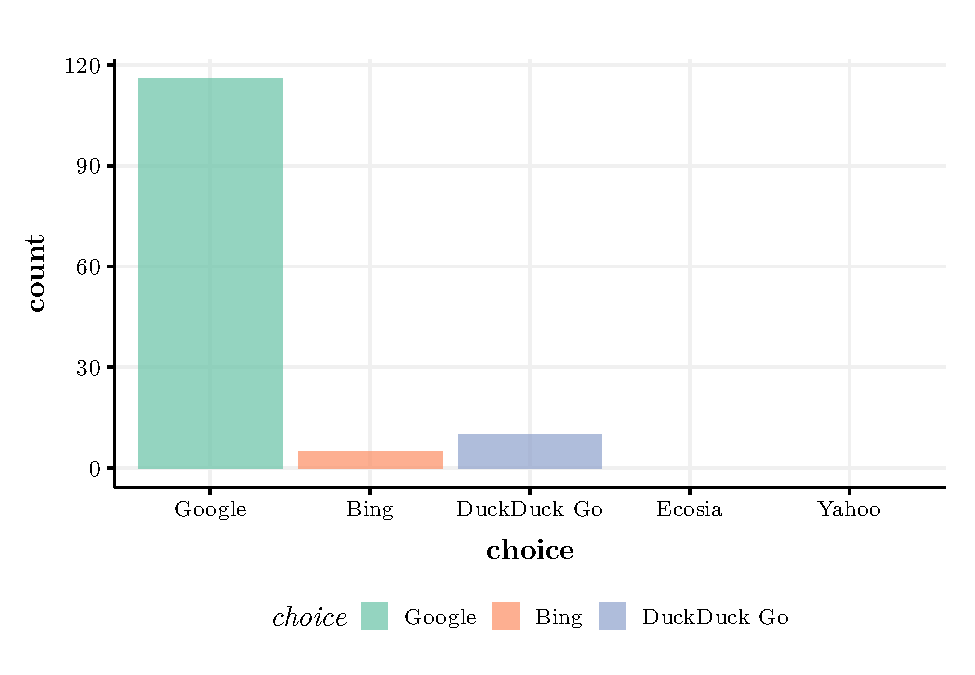
\includegraphics{analysis-July19_files/figure-latex/unnamed-chunk-9-1.pdf}

\begin{Shaded}
\begin{Highlighting}[]
\CommentTok{\# test = dfexp \%\textgreater{}\% }
\CommentTok{\#   mutate(across(starts\_with("used"), as.numeric)) }

\CommentTok{\#\textquotesingle{} *This worked!!! Saves a lot of time. Mind I should use "across" much more. And apply, lapply, sapply too.*}

\CommentTok{\# test = test \%\textgreater{}\% }
\CommentTok{\#   mutate(nbing = used\_bing\_q1 + used\_bing\_q2 + used\_bing\_q3) \# This works too!}
\end{Highlighting}
\end{Shaded}

\hypertarget{creates-dfs-for-comparison-pada-vs-pac}{%
\subsection{creates dfs for comparison pA\textbar D(A) vs pA\textbar C}\label{creates-dfs-for-comparison-pada-vs-pac}}

\begin{Shaded}
\begin{Highlighting}[]
\CommentTok{\# Create dfs for comparison with forced choice}

\NormalTok{dfgoogle }\OtherTok{=}\NormalTok{ dfexp }\SpecialCharTok{\%\textgreater{}\%} 
  \FunctionTok{filter}\NormalTok{(forced\_choice\_s}\SpecialCharTok{==}\DecValTok{1} \SpecialCharTok{|}\NormalTok{ assigned\_google}\SpecialCharTok{==}\DecValTok{1}\NormalTok{) }

\NormalTok{dfbing }\OtherTok{=}\NormalTok{ dfexp }\SpecialCharTok{\%\textgreater{}\%} 
  \FunctionTok{filter}\NormalTok{(forced\_choice\_s}\SpecialCharTok{==}\DecValTok{1} \SpecialCharTok{|}\NormalTok{ assigned\_bing}\SpecialCharTok{==}\DecValTok{1}\NormalTok{) }

\NormalTok{dfyahoo }\OtherTok{=}\NormalTok{ dfexp }\SpecialCharTok{\%\textgreater{}\%} 
  \FunctionTok{filter}\NormalTok{(forced\_choice\_s}\SpecialCharTok{==}\DecValTok{1} \SpecialCharTok{|}\NormalTok{ assigned\_yahoo}\SpecialCharTok{==}\DecValTok{1}\NormalTok{) }

\NormalTok{dfddg }\OtherTok{=}\NormalTok{ dfexp }\SpecialCharTok{\%\textgreater{}\%} 
  \FunctionTok{filter}\NormalTok{(forced\_choice\_s}\SpecialCharTok{==}\DecValTok{1} \SpecialCharTok{|}\NormalTok{ assigned\_duckduckgo}\SpecialCharTok{==}\DecValTok{1}\NormalTok{) }
\end{Highlighting}
\end{Shaded}

\begin{Shaded}
\begin{Highlighting}[]
\FunctionTok{library}\NormalTok{(jtools)}
\end{Highlighting}
\end{Shaded}

Mind there are two ways to operationalize the effect:

\begin{enumerate}
\def\labelenumi{\arabic{enumi})}
\item
  compared with choice-screen
\item
  compared with any other default
\end{enumerate}

\hypertarget{creates-df-for-default-condition}{%
\subsection{creates df for default condition}\label{creates-df-for-default-condition}}

\begin{Shaded}
\begin{Highlighting}[]
\CommentTok{\# DF for defaults in search}
\NormalTok{dfexp\_def\_s }\OtherTok{=}\NormalTok{ dfexp }\SpecialCharTok{\%\textgreater{}\%} 
  \FunctionTok{filter}\NormalTok{(choice\_search}\SpecialCharTok{==}\DecValTok{0}\NormalTok{)}
\end{Highlighting}
\end{Shaded}

\hypertarget{status-quo-effects-search}{%
\section{Status Quo Effects Search}\label{status-quo-effects-search}}

\hypertarget{bing}{%
\subsection{Bing}\label{bing}}

\begin{Shaded}
\begin{Highlighting}[]
\CommentTok{\# Bing Q1}
\NormalTok{sqbingq1}\OtherTok{=} \FunctionTok{glm}\NormalTok{(used\_bing\_q1 }\SpecialCharTok{\textasciitilde{}}\NormalTok{ forced\_choice\_s, }\AttributeTok{data=}\NormalTok{dfbing, }\AttributeTok{family =}\StringTok{"binomial"}\NormalTok{)}

\CommentTok{\#check effect on quality}

\NormalTok{qualbing }\OtherTok{=} \FunctionTok{lm}\NormalTok{(bing\_qual }\SpecialCharTok{\textasciitilde{}}\NormalTok{ forced\_choice\_s, }\AttributeTok{data =}\NormalTok{ dfbing)}

\FunctionTok{summary}\NormalTok{(qualbing)}
\end{Highlighting}
\end{Shaded}

\begin{verbatim}
## 
## Call:
## lm(formula = bing_qual ~ forced_choice_s, data = dfbing)
## 
## Residuals:
##     Min      1Q  Median      3Q     Max 
## -2.8929 -0.7689  0.0471  0.8012  2.2311 
## 
## Coefficients:
##                  Estimate Std. Error t value             Pr(>|t|)    
## (Intercept)        3.5729     0.2024  17.657 < 0.0000000000000002 ***
## forced_choice_s1  -0.8040     0.2250  -3.573             0.000466 ***
## ---
## Signif. codes:  0 '***' 0.001 '**' 0.01 '*' 0.05 '.' 0.1 ' ' 1
## 
## Residual standard error: 1.127 on 160 degrees of freedom
## Multiple R-squared:  0.0739, Adjusted R-squared:  0.06811 
## F-statistic: 12.77 on 1 and 160 DF,  p-value: 0.0004664
\end{verbatim}

\begin{Shaded}
\begin{Highlighting}[]
\NormalTok{plotbingq1 }\OtherTok{=} \FunctionTok{effect\_plot}\NormalTok{(sqbingq1, }\AttributeTok{pred =} \StringTok{"forced\_choice\_s"}\NormalTok{, }\AttributeTok{interval =} \ConstantTok{TRUE}\NormalTok{, }\AttributeTok{plot.points =} \ConstantTok{TRUE}\NormalTok{, }\AttributeTok{jitter =} \FunctionTok{c}\NormalTok{(}\FloatTok{0.2}\NormalTok{, }\FloatTok{0.01}\NormalTok{), }\AttributeTok{point.alpha =} \FloatTok{0.4}\NormalTok{, }\AttributeTok{colors =} \StringTok{"Qual1"}\NormalTok{)}

\NormalTok{plotbingq1}
\end{Highlighting}
\end{Shaded}

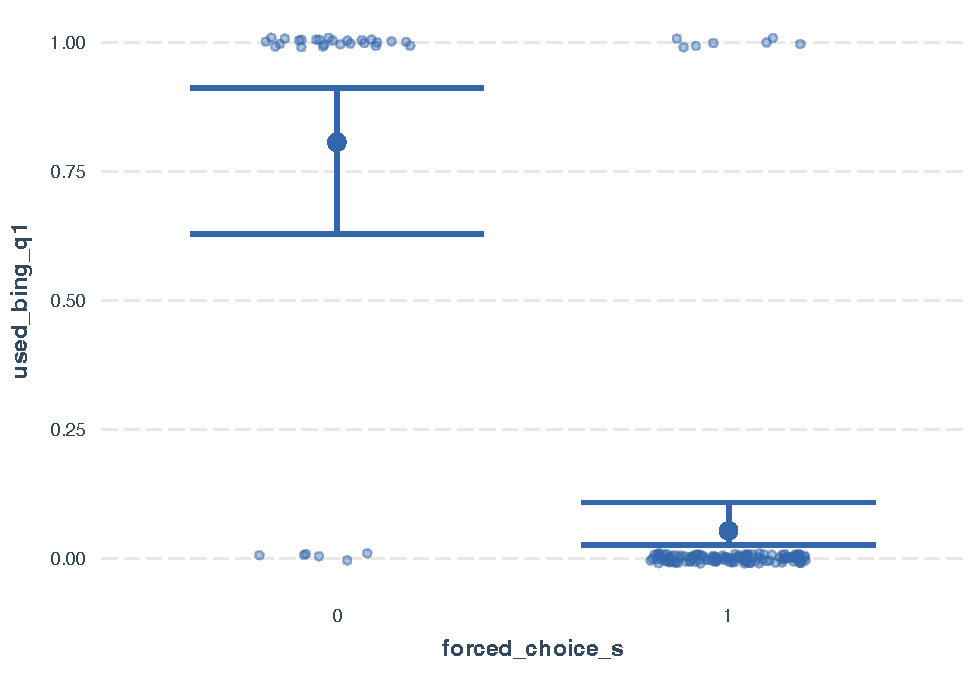
\includegraphics{analysis-July19_files/figure-latex/unnamed-chunk-14-1.pdf}

*Interesting. Status quo effect goes down. People start switching. I need longer questionnaire. Hopefully, 5 enough. If not, run final version with 7 questions? Not sure it's worth it

*Different comparison: Pb\textbar B compared with any other default

\begin{Shaded}
\begin{Highlighting}[]
\FunctionTok{lm}\NormalTok{(}\AttributeTok{data =}\NormalTok{ dfexp, used\_bing\_q1 }\SpecialCharTok{\textasciitilde{}}\NormalTok{ assigned\_bing)}
\end{Highlighting}
\end{Shaded}

\begin{verbatim}
## 
## Call:
## lm(formula = used_bing_q1 ~ assigned_bing, data = dfexp)
## 
## Coefficients:
##    (Intercept)  assigned_bing1  
##        0.01053         0.79593
\end{verbatim}

\begin{Shaded}
\begin{Highlighting}[]
\FunctionTok{lm}\NormalTok{(}\AttributeTok{data =}\NormalTok{ dfexp, used\_bing\_q1 }\SpecialCharTok{\textasciitilde{}}\NormalTok{ assigned\_bing }\SpecialCharTok{+}\NormalTok{ bing\_qual }\SpecialCharTok{+}\NormalTok{ bing\_prior) }\CommentTok{\#It is working this time! Gather larger n too. But quality and prior use are correlated and my sample is not }
\end{Highlighting}
\end{Shaded}

\begin{verbatim}
## 
## Call:
## lm(formula = used_bing_q1 ~ assigned_bing + bing_qual + bing_prior, 
##     data = dfexp)
## 
## Coefficients:
##    (Intercept)  assigned_bing1       bing_qual      bing_prior  
##       -0.19284         0.73993         0.07055         0.01190
\end{verbatim}

\begin{Shaded}
\begin{Highlighting}[]
\NormalTok{bingq1 }\OtherTok{=} \FunctionTok{glm}\NormalTok{(}\AttributeTok{data =}\NormalTok{ dfexp\_def\_s, used\_bing\_q1 }\SpecialCharTok{\textasciitilde{}}\NormalTok{ assigned\_bing}\SpecialCharTok{:}\NormalTok{ bing\_prior, }\AttributeTok{family =} \StringTok{"binomial"}\NormalTok{)}

\FunctionTok{summary}\NormalTok{(bingq1)}
\end{Highlighting}
\end{Shaded}

\begin{verbatim}
## 
## Call:
## glm(formula = used_bing_q1 ~ assigned_bing:bing_prior, family = "binomial", 
##     data = dfexp_def_s)
## 
## Coefficients:
##                           Estimate Std. Error z value    Pr(>|z|)    
## (Intercept)                -1.9636     0.3775  -5.201 0.000000198 ***
## assigned_bing0:bing_prior  -1.7500     1.0802  -1.620       0.105    
## assigned_bing1:bing_prior   4.1037     0.8375   4.900 0.000000958 ***
## ---
## Signif. codes:  0 '***' 0.001 '**' 0.01 '*' 0.05 '.' 0.1 ' ' 1
## 
## (Dispersion parameter for binomial family taken to be 1)
## 
##     Null deviance: 128.29  on 125  degrees of freedom
## Residual deviance:  70.73  on 123  degrees of freedom
## AIC: 76.73
## 
## Number of Fisher Scoring iterations: 6
\end{verbatim}

\begin{Shaded}
\begin{Highlighting}[]
\FunctionTok{typeof}\NormalTok{(dfexp}\SpecialCharTok{$}\NormalTok{bing\_qual)}
\end{Highlighting}
\end{Shaded}

\begin{verbatim}
## [1] "double"
\end{verbatim}

\begin{Shaded}
\begin{Highlighting}[]
\FunctionTok{lm}\NormalTok{(}\AttributeTok{data =}\NormalTok{ dfexp, used\_bing\_q3 }\SpecialCharTok{\textasciitilde{}}\NormalTok{ assigned\_bing)}
\end{Highlighting}
\end{Shaded}

\begin{verbatim}
## 
## Call:
## lm(formula = used_bing_q3 ~ assigned_bing, data = dfexp)
## 
## Coefficients:
##    (Intercept)  assigned_bing1  
##        0.01053         0.66689
\end{verbatim}

\begin{Shaded}
\begin{Highlighting}[]
\CommentTok{\#\textquotesingle{}* Second experiment*}
\FunctionTok{lm}\NormalTok{(}\AttributeTok{data =}\NormalTok{ datexp, used\_bing\_q1 }\SpecialCharTok{\textasciitilde{}}\NormalTok{ assigned\_bing)}
\end{Highlighting}
\end{Shaded}

\begin{verbatim}
## 
## Call:
## lm(formula = used_bing_q1 ~ assigned_bing, data = datexp)
## 
## Coefficients:
##    (Intercept)  assigned_bing1  
##        0.03086         0.72710
\end{verbatim}

\begin{Shaded}
\begin{Highlighting}[]
\NormalTok{e2.test }\OtherTok{=} \FunctionTok{lm}\NormalTok{(}\AttributeTok{data =}\NormalTok{ datexp, used\_bing\_q1 }\SpecialCharTok{\textasciitilde{}}\NormalTok{ assigned\_bing}\SpecialCharTok{:}\NormalTok{bing\_prior }\SpecialCharTok{+}\NormalTok{ bing\_qual)}
\FunctionTok{summary}\NormalTok{(e2.test) }\CommentTok{\#there is an interaction effect. Prior use moderates the effect of the default}
\end{Highlighting}
\end{Shaded}

\begin{verbatim}
## 
## Call:
## lm(formula = used_bing_q1 ~ assigned_bing:bing_prior + bing_qual, 
##     data = datexp)
## 
## Residuals:
##      Min       1Q   Median       3Q      Max 
## -0.87099 -0.15981 -0.07405  0.16978  0.92608 
## 
## Coefficients:
##                           Estimate Std. Error t value            Pr(>|t|)    
## (Intercept)                0.05064    0.06301   0.804              0.4222    
## bing_qual                  0.03988    0.01970   2.024              0.0439 *  
## assigned_bing0:bing_prior -0.11669    0.05617  -2.078              0.0386 *  
## assigned_bing1:bing_prior  0.62096    0.04936  12.581 <0.0000000000000002 ***
## ---
## Signif. codes:  0 '***' 0.001 '**' 0.01 '*' 0.05 '.' 0.1 ' ' 1
## 
## Residual standard error: 0.3547 on 310 degrees of freedom
##   (5 observations deleted due to missingness)
## Multiple R-squared:  0.4802, Adjusted R-squared:  0.4752 
## F-statistic: 95.46 on 3 and 310 DF,  p-value: < 0.00000000000000022
\end{verbatim}

\begin{Shaded}
\begin{Highlighting}[]
\NormalTok{e2.bingq1 }\OtherTok{=} \FunctionTok{glm}\NormalTok{(}\AttributeTok{data =}\NormalTok{ datexp, used\_bing\_q1 }\SpecialCharTok{\textasciitilde{}}\NormalTok{ assigned\_bing }\SpecialCharTok{+}\NormalTok{ bing\_prior, }\AttributeTok{family =} \StringTok{"binomial"}\NormalTok{)}

\FunctionTok{summary}\NormalTok{(e2.bingq1)}
\end{Highlighting}
\end{Shaded}

\begin{verbatim}
## 
## Call:
## glm(formula = used_bing_q1 ~ assigned_bing + bing_prior, family = "binomial", 
##     data = datexp)
## 
## Coefficients:
##                Estimate Std. Error z value             Pr(>|z|)    
## (Intercept)     -4.3456     0.5390  -8.062 0.000000000000000752 ***
## assigned_bing1   4.4281     0.5000   8.857 < 0.0000000000000002 ***
## bing_prior       1.5298     0.3801   4.024 0.000057136630600006 ***
## ---
## Signif. codes:  0 '***' 0.001 '**' 0.01 '*' 0.05 '.' 0.1 ' ' 1
## 
## (Dispersion parameter for binomial family taken to be 1)
## 
##     Null deviance: 426.29  on 318  degrees of freedom
## Residual deviance: 201.80  on 316  degrees of freedom
## AIC: 207.8
## 
## Number of Fisher Scoring iterations: 6
\end{verbatim}

\begin{Shaded}
\begin{Highlighting}[]
\CommentTok{\#\textquotesingle{}*visualization*}
\CommentTok{\# E2. Bing Q1}
\NormalTok{e2.sqbingq1}\OtherTok{=} \FunctionTok{glm}\NormalTok{(used\_bing\_q1 }\SpecialCharTok{\textasciitilde{}}\NormalTok{ assigned\_bing, }\AttributeTok{data=}\NormalTok{datexp, }\AttributeTok{family =}\StringTok{"binomial"}\NormalTok{)}

\NormalTok{e2.plotbingq1 }\OtherTok{=} \FunctionTok{effect\_plot}\NormalTok{(e2.sqbingq1, }\AttributeTok{pred =} \StringTok{"assigned\_bing"}\NormalTok{, }\AttributeTok{interval =} \ConstantTok{TRUE}\NormalTok{, }\AttributeTok{plot.points =} \ConstantTok{TRUE}\NormalTok{, }\AttributeTok{jitter =} \FunctionTok{c}\NormalTok{(}\FloatTok{0.2}\NormalTok{, }\FloatTok{0.01}\NormalTok{), }\AttributeTok{point.alpha =} \FloatTok{0.4}\NormalTok{, }\AttributeTok{colors =} \StringTok{"Qual1"}\NormalTok{)}

\NormalTok{e2.plotbingq1}
\end{Highlighting}
\end{Shaded}

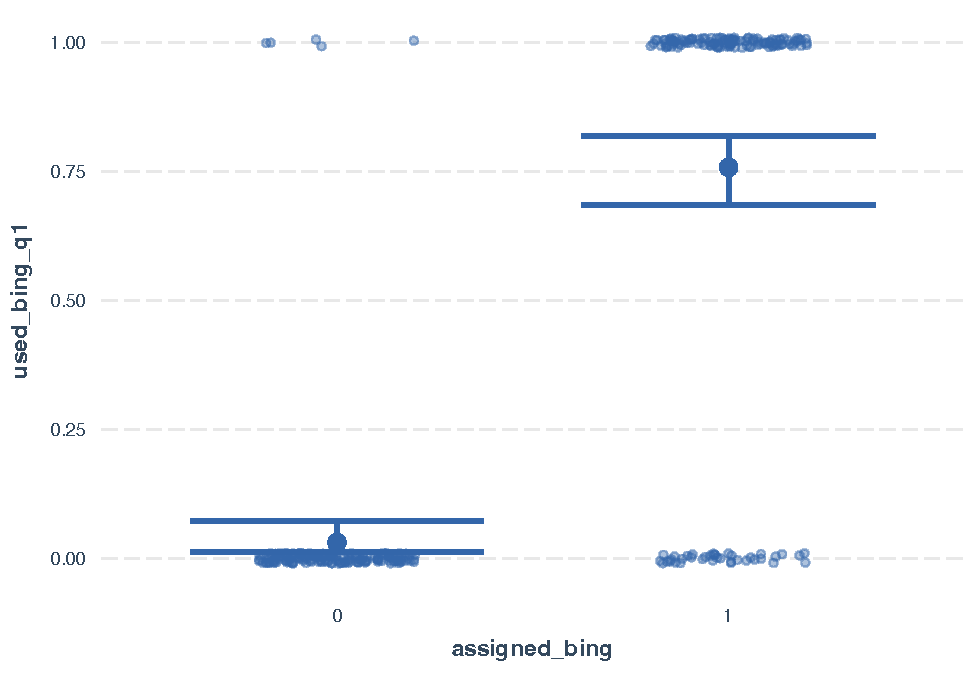
\includegraphics{analysis-July19_files/figure-latex/unnamed-chunk-16-1.pdf}

Now, do the same for Q5

\begin{Shaded}
\begin{Highlighting}[]
\NormalTok{e2.sqbingq5}\OtherTok{=} \FunctionTok{glm}\NormalTok{(used\_bing\_q5 }\SpecialCharTok{\textasciitilde{}}\NormalTok{ assigned\_bing, }\AttributeTok{data=}\NormalTok{datexp, }\AttributeTok{family =}\StringTok{"binomial"}\NormalTok{)}

\NormalTok{e2.plotbingq5 }\OtherTok{=} \FunctionTok{effect\_plot}\NormalTok{(e2.sqbingq5, }\AttributeTok{pred =} \StringTok{"assigned\_bing"}\NormalTok{, }\AttributeTok{interval =} \ConstantTok{TRUE}\NormalTok{, }\AttributeTok{plot.points =} \ConstantTok{TRUE}\NormalTok{, }\AttributeTok{jitter =} \FunctionTok{c}\NormalTok{(}\FloatTok{0.2}\NormalTok{, }\FloatTok{0.01}\NormalTok{), }\AttributeTok{point.alpha =} \FloatTok{0.4}\NormalTok{, }\AttributeTok{colors =} \StringTok{"Qual1"}\NormalTok{)}

\NormalTok{e2.plotbingq5}
\end{Highlighting}
\end{Shaded}

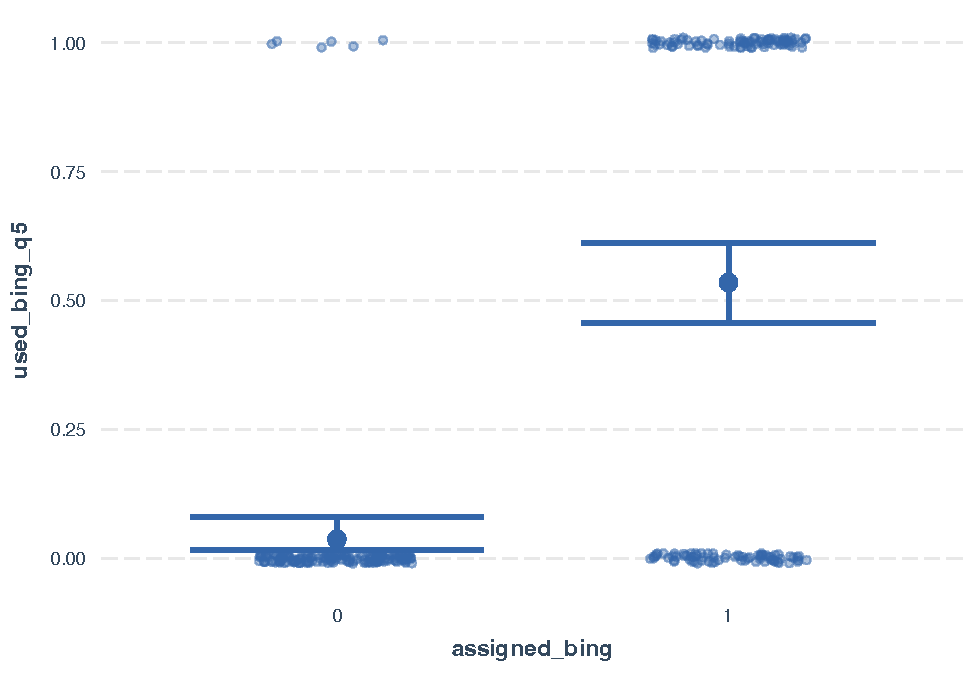
\includegraphics{analysis-July19_files/figure-latex/unnamed-chunk-17-1.pdf}

See how this effect affects Google

\hypertarget{video-had-no-effect.-probably-everyone-pais-attention.-check-number-of-correct-answers}{%
\subsection{Video had no effect. Probably everyone pais attention. Check number of correct answers}\label{video-had-no-effect.-probably-everyone-pais-attention.-check-number-of-correct-answers}}

See if video had an effect\ldots{} It did not work out. No difference

\begin{Shaded}
\begin{Highlighting}[]
\CommentTok{\# Creates status quo variable (for Q1)}
\NormalTok{datexp }\OtherTok{=}\NormalTok{ datexp }\SpecialCharTok{\%\textgreater{}\%} 
  \FunctionTok{mutate}\NormalTok{(}\AttributeTok{statquo =} \FunctionTok{ifelse}\NormalTok{(assigned\_bing }\SpecialCharTok{==}\DecValTok{1} \SpecialCharTok{\&}\NormalTok{ used\_bing\_q1}\SpecialCharTok{==}\DecValTok{1} \SpecialCharTok{|}\NormalTok{ assigned\_google }\SpecialCharTok{==}\DecValTok{1} \SpecialCharTok{\&}\NormalTok{ used\_google\_q1}\SpecialCharTok{==}\DecValTok{1}\NormalTok{, }\DecValTok{1}\NormalTok{,}\DecValTok{0}\NormalTok{),}
         \AttributeTok{video =} \FunctionTok{as.factor}\NormalTok{(video))}

\FunctionTok{mean}\NormalTok{(datexp}\SpecialCharTok{$}\NormalTok{statquo)}
\end{Highlighting}
\end{Shaded}

\begin{verbatim}
## [1] 0.8526646
\end{verbatim}

\begin{Shaded}
\begin{Highlighting}[]
\NormalTok{datbing }\OtherTok{=}\NormalTok{ datexp }\SpecialCharTok{\%\textgreater{}\%} 
  \FunctionTok{filter}\NormalTok{(assigned\_bing}\SpecialCharTok{==}\DecValTok{1}\NormalTok{) }\CommentTok{\# New DF to compare just those assigned to Bing}

\NormalTok{glmvideo }\OtherTok{=} \FunctionTok{glm}\NormalTok{(}\AttributeTok{data=}\NormalTok{datexp, }\AttributeTok{formula=}\NormalTok{statquo }\SpecialCharTok{\textasciitilde{}}\NormalTok{ video, }\AttributeTok{family =} \StringTok{"binomial"}\NormalTok{)}

\FunctionTok{summary}\NormalTok{(glmvideo)}
\end{Highlighting}
\end{Shaded}

\begin{verbatim}
## 
## Call:
## glm(formula = statquo ~ video, family = "binomial", data = datexp)
## 
## Coefficients:
##             Estimate Std. Error z value            Pr(>|z|)    
## (Intercept)   2.0323     0.2440    8.33 <0.0000000000000002 ***
## video1       -0.5203     0.3211   -1.62               0.105    
## ---
## Signif. codes:  0 '***' 0.001 '**' 0.01 '*' 0.05 '.' 0.1 ' ' 1
## 
## (Dispersion parameter for binomial family taken to be 1)
## 
##     Null deviance: 266.72  on 318  degrees of freedom
## Residual deviance: 264.05  on 317  degrees of freedom
## AIC: 268.05
## 
## Number of Fisher Scoring iterations: 4
\end{verbatim}

\begin{Shaded}
\begin{Highlighting}[]
\NormalTok{glm.video }\OtherTok{=} \FunctionTok{effect\_plot}\NormalTok{(glmvideo, }\AttributeTok{pred =} \StringTok{"video"}\NormalTok{, }\AttributeTok{interval =} \ConstantTok{TRUE}\NormalTok{, }\AttributeTok{plot.points =} \ConstantTok{TRUE}\NormalTok{, }\AttributeTok{jitter =} \FunctionTok{c}\NormalTok{(}\FloatTok{0.2}\NormalTok{, }\FloatTok{0.01}\NormalTok{), }\AttributeTok{point.alpha =} \FloatTok{0.4}\NormalTok{, }\AttributeTok{colors =} \StringTok{"Qual1"}\NormalTok{)}

\NormalTok{glm.video}
\end{Highlighting}
\end{Shaded}

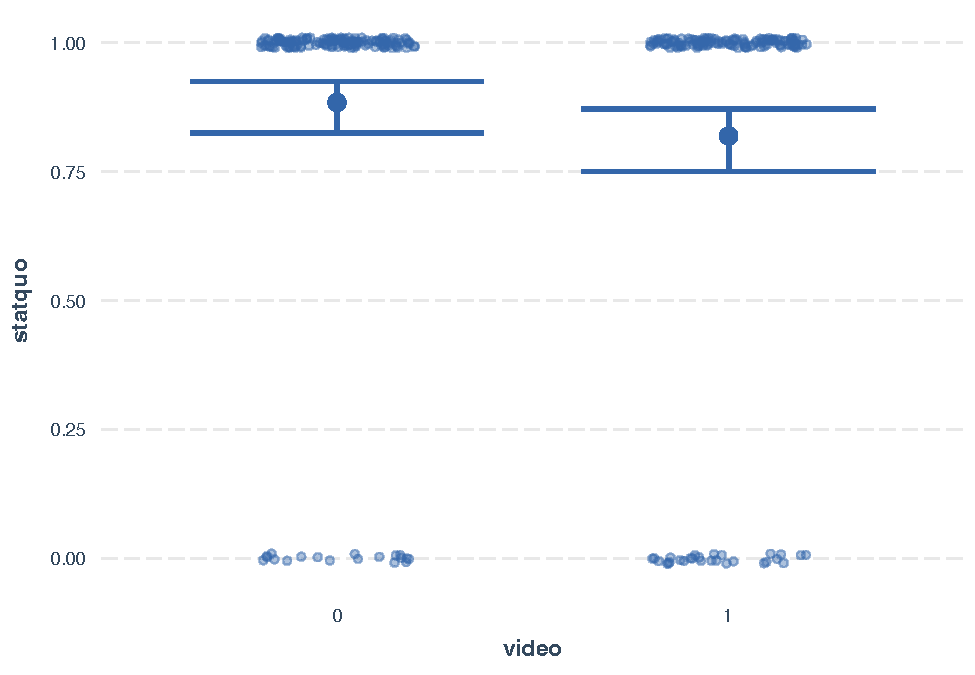
\includegraphics{analysis-July19_files/figure-latex/unnamed-chunk-18-1.pdf}

\begin{Shaded}
\begin{Highlighting}[]
\NormalTok{e2.googleq5}\OtherTok{=} \FunctionTok{glm}\NormalTok{(used\_google\_q5 }\SpecialCharTok{\textasciitilde{}}\NormalTok{ assigned\_bing, }\AttributeTok{data=}\NormalTok{datexp, }\AttributeTok{family =}\StringTok{"binomial"}\NormalTok{)}

\NormalTok{e2.plotgoogleq5 }\OtherTok{=} \FunctionTok{effect\_plot}\NormalTok{(e2.googleq5, }\AttributeTok{pred =} \StringTok{"assigned\_bing"}\NormalTok{, }\AttributeTok{interval =} \ConstantTok{TRUE}\NormalTok{, }\AttributeTok{plot.points =} \ConstantTok{TRUE}\NormalTok{, }\AttributeTok{jitter =} \FunctionTok{c}\NormalTok{(}\FloatTok{0.2}\NormalTok{, }\FloatTok{0.01}\NormalTok{), }\AttributeTok{point.alpha =} \FloatTok{0.4}\NormalTok{, }\AttributeTok{colors =} \StringTok{"Qual1"}\NormalTok{)}

\NormalTok{e2.plotgoogleq5}
\end{Highlighting}
\end{Shaded}

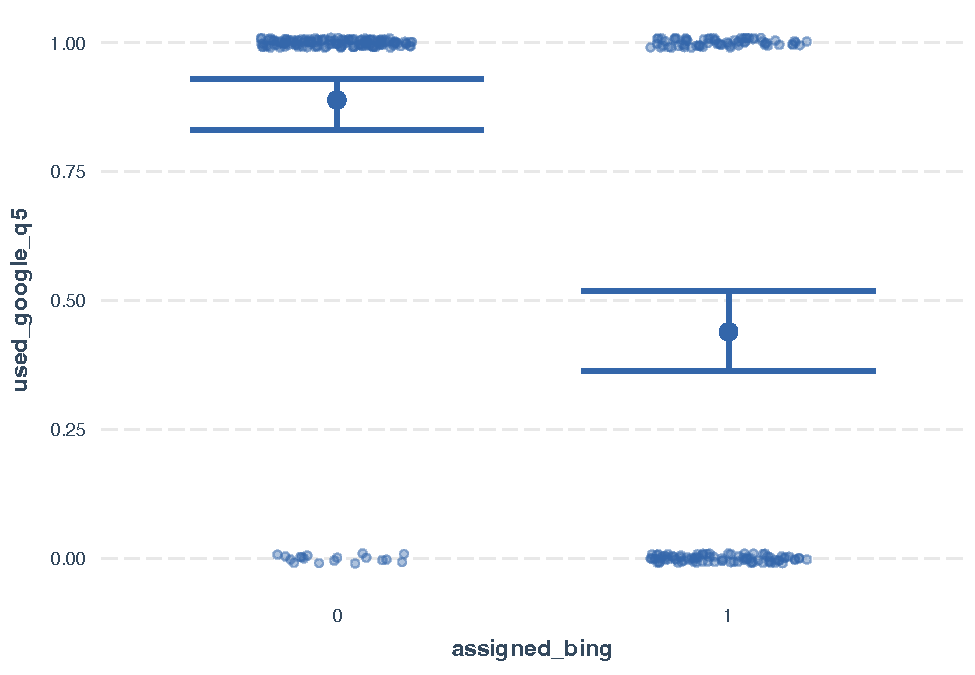
\includegraphics{analysis-July19_files/figure-latex/unnamed-chunk-19-1.pdf}
Substantial effect! lowers use of Google!

\begin{Shaded}
\begin{Highlighting}[]
\CommentTok{\#Bing Q3}

\NormalTok{sqbingq3}\OtherTok{=} \FunctionTok{glm}\NormalTok{(used\_bing\_q3 }\SpecialCharTok{\textasciitilde{}}\NormalTok{ forced\_choice\_s, }\AttributeTok{data=}\NormalTok{dfbing, }\AttributeTok{family =}\StringTok{"binomial"}\NormalTok{)}

\NormalTok{plotbingq3 }\OtherTok{=} \FunctionTok{effect\_plot}\NormalTok{(sqbingq3, }\AttributeTok{pred =} \StringTok{"forced\_choice\_s"}\NormalTok{, }\AttributeTok{interval =} \ConstantTok{TRUE}\NormalTok{, }\AttributeTok{plot.points =} \ConstantTok{TRUE}\NormalTok{, }\AttributeTok{jitter =} \FunctionTok{c}\NormalTok{(}\FloatTok{0.2}\NormalTok{, }\FloatTok{0.01}\NormalTok{), }\AttributeTok{point.alpha =} \FloatTok{0.4}\NormalTok{, }\AttributeTok{colors =} \StringTok{"Qual1"}\NormalTok{)}

\NormalTok{plotbingq3}
\end{Highlighting}
\end{Shaded}

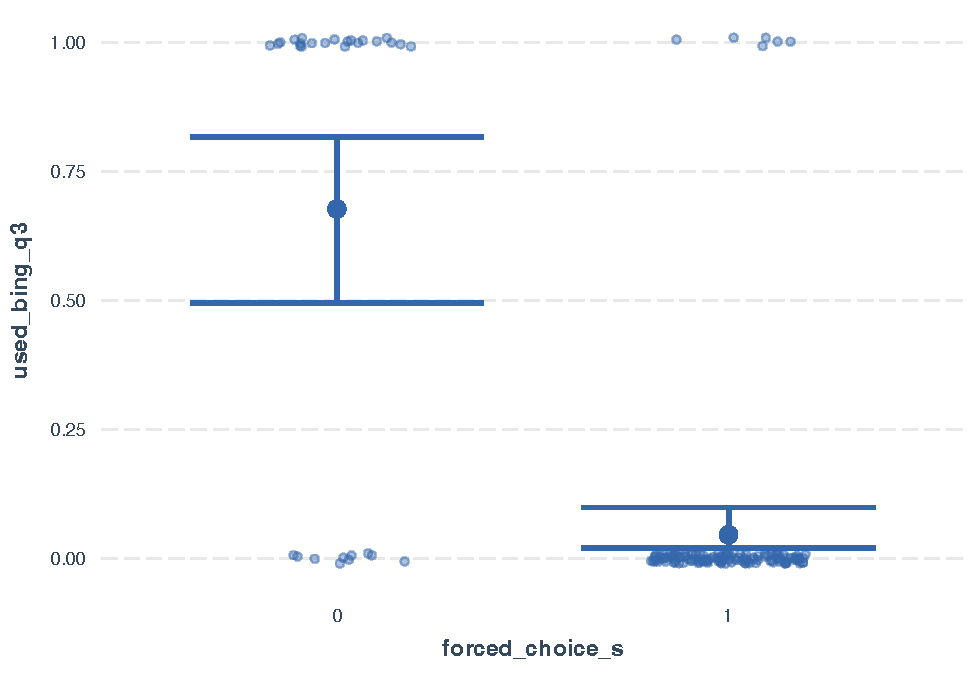
\includegraphics{analysis-July19_files/figure-latex/unnamed-chunk-20-1.pdf}

\hypertarget{yahoo}{%
\subsection{Yahoo}\label{yahoo}}

Check status quo effects for Yahoo. There is no variance, so just report counts

\begin{Shaded}
\begin{Highlighting}[]
\NormalTok{sqyahooq1}\OtherTok{=} \FunctionTok{glm}\NormalTok{(used\_yahoo\_q1 }\SpecialCharTok{\textasciitilde{}}\NormalTok{ forced\_choice\_s, }\AttributeTok{data=}\NormalTok{dfyahoo, }\AttributeTok{family =}\StringTok{"binomial"}\NormalTok{)}


\NormalTok{plotyahooq1 }\OtherTok{=} \FunctionTok{effect\_plot}\NormalTok{(sqyahooq1, }\AttributeTok{pred =} \StringTok{"forced\_choice\_s"}\NormalTok{, }\AttributeTok{interval =} \ConstantTok{TRUE}\NormalTok{, }\AttributeTok{plot.points =} \ConstantTok{TRUE}\NormalTok{, }\AttributeTok{jitter =} \FunctionTok{c}\NormalTok{(}\FloatTok{0.2}\NormalTok{, }\FloatTok{0.01}\NormalTok{), }\AttributeTok{point.alpha =} \FloatTok{0.4}\NormalTok{, }\AttributeTok{colors =} \StringTok{"Qual1"}\NormalTok{)}


\CommentTok{\#Now check for default data: pY|Y vs pY|Y\textasciigrave{}}

\NormalTok{sqdefyahooq1 }\OtherTok{=} \FunctionTok{glm}\NormalTok{(used\_yahoo\_q1 }\SpecialCharTok{\textasciitilde{}}\NormalTok{ assigned\_yahoo, }\AttributeTok{data=}\NormalTok{dfexp\_def\_s, }\AttributeTok{family =}\StringTok{"binomial"}\NormalTok{)}

\NormalTok{plotsqdefyahooq1 }\OtherTok{=} \FunctionTok{effect\_plot}\NormalTok{(sqdefyahooq1, }\AttributeTok{pred =} \StringTok{"assigned\_yahoo"}\NormalTok{, }\AttributeTok{interval =} \ConstantTok{TRUE}\NormalTok{, }\AttributeTok{plot.points =} \ConstantTok{TRUE}\NormalTok{, }\AttributeTok{jitter =} \FunctionTok{c}\NormalTok{(}\FloatTok{0.2}\NormalTok{, }\FloatTok{0.01}\NormalTok{), }\AttributeTok{point.alpha =} \FloatTok{0.4}\NormalTok{, }\AttributeTok{colors =} \StringTok{"Qual1"}\NormalTok{)}

\CommentTok{\# Check q3}

\NormalTok{sqdefyahooq3 }\OtherTok{=} \FunctionTok{glm}\NormalTok{(used\_yahoo\_q3 }\SpecialCharTok{\textasciitilde{}}\NormalTok{ assigned\_yahoo, }\AttributeTok{data=}\NormalTok{dfexp\_def\_s, }\AttributeTok{family =}\StringTok{"binomial"}\NormalTok{)}

\NormalTok{plotsqdefyahooq3 }\OtherTok{=} \FunctionTok{effect\_plot}\NormalTok{(sqdefyahooq3, }\AttributeTok{pred =} \StringTok{"assigned\_yahoo"}\NormalTok{, }\AttributeTok{interval =} \ConstantTok{TRUE}\NormalTok{, }\AttributeTok{plot.points =} \ConstantTok{TRUE}\NormalTok{, }\AttributeTok{jitter =} \FunctionTok{c}\NormalTok{(}\FloatTok{0.2}\NormalTok{, }\FloatTok{0.01}\NormalTok{), }\AttributeTok{point.alpha =} \FloatTok{0.4}\NormalTok{, }\AttributeTok{colors =} \StringTok{"Qual1"}\NormalTok{)}

\NormalTok{plotyahooq1}
\end{Highlighting}
\end{Shaded}

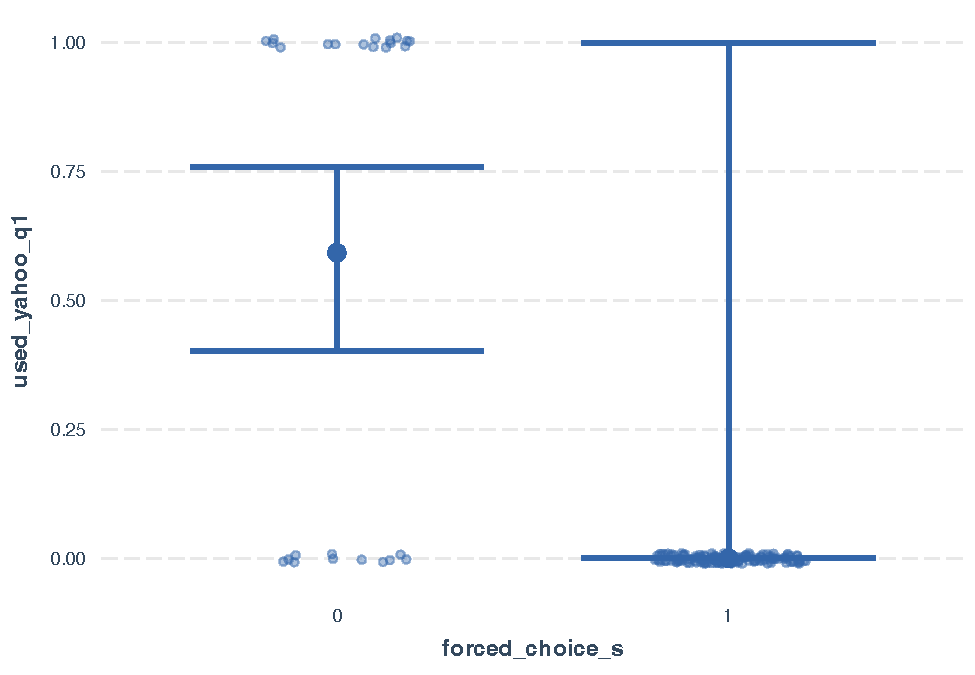
\includegraphics{analysis-July19_files/figure-latex/unnamed-chunk-21-1.pdf}

\begin{Shaded}
\begin{Highlighting}[]
\NormalTok{plotsqdefyahooq1}
\end{Highlighting}
\end{Shaded}

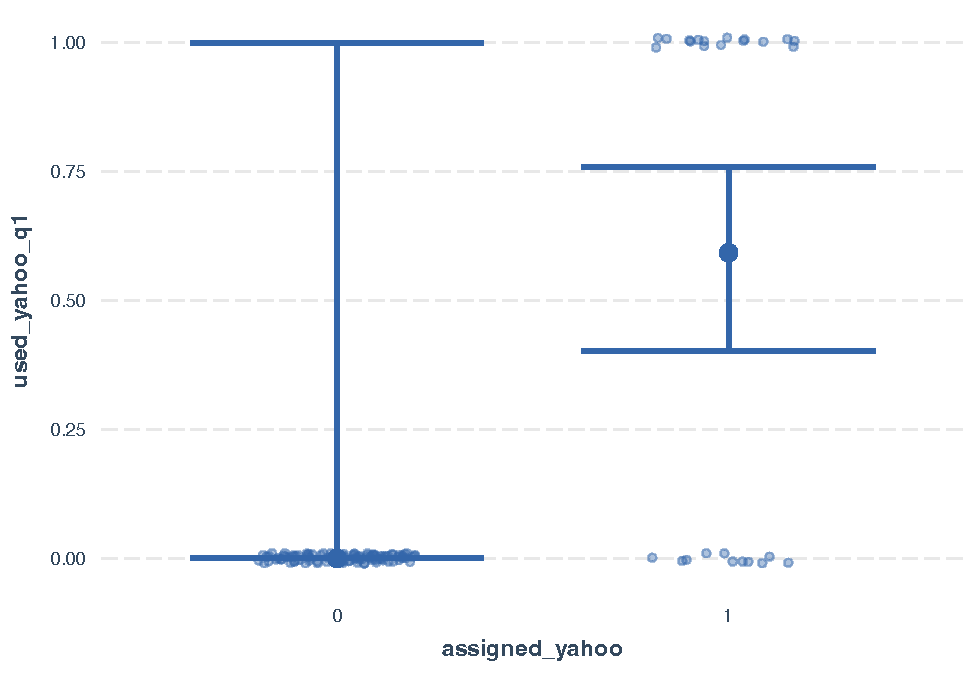
\includegraphics{analysis-July19_files/figure-latex/unnamed-chunk-21-2.pdf}

\begin{Shaded}
\begin{Highlighting}[]
\NormalTok{plotsqdefyahooq3}
\end{Highlighting}
\end{Shaded}

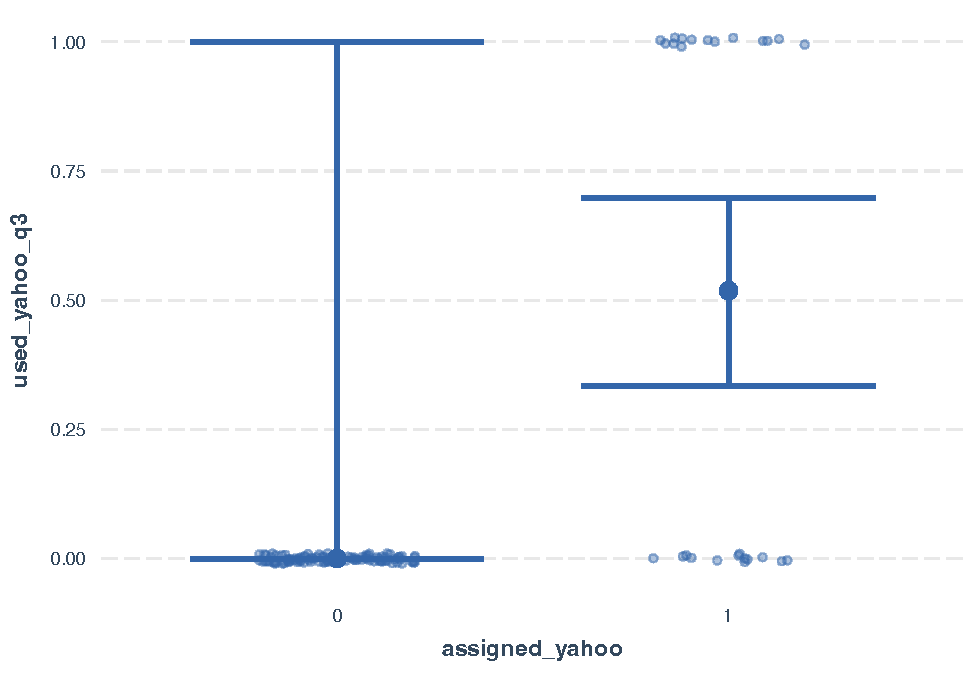
\includegraphics{analysis-July19_files/figure-latex/unnamed-chunk-21-3.pdf}

\hypertarget{duckduck-go}{%
\subsection{DuckDuck Go}\label{duckduck-go}}

Do the same with DuckDuckGo

\begin{Shaded}
\begin{Highlighting}[]
\NormalTok{sqdefddg1 }\OtherTok{=} \FunctionTok{glm}\NormalTok{(used\_duckduckgo\_q1 }\SpecialCharTok{\textasciitilde{}}\NormalTok{ assigned\_duckduckgo, }\AttributeTok{data=}\NormalTok{dfexp\_def\_s, }\AttributeTok{family =}\StringTok{"binomial"}\NormalTok{)}

\NormalTok{plotsqdefddg1 }\OtherTok{=} \FunctionTok{effect\_plot}\NormalTok{(sqdefddg1, }\AttributeTok{pred =} \StringTok{"assigned\_duckduckgo"}\NormalTok{, }\AttributeTok{interval =} \ConstantTok{TRUE}\NormalTok{, }\AttributeTok{plot.points =} \ConstantTok{TRUE}\NormalTok{, }\AttributeTok{jitter =} \FunctionTok{c}\NormalTok{(}\FloatTok{0.2}\NormalTok{, }\FloatTok{0.01}\NormalTok{), }\AttributeTok{point.alpha =} \FloatTok{0.4}\NormalTok{, }\AttributeTok{colors =} \StringTok{"Qual1"}\NormalTok{)}

\NormalTok{plotsqdefddg1}
\end{Highlighting}
\end{Shaded}

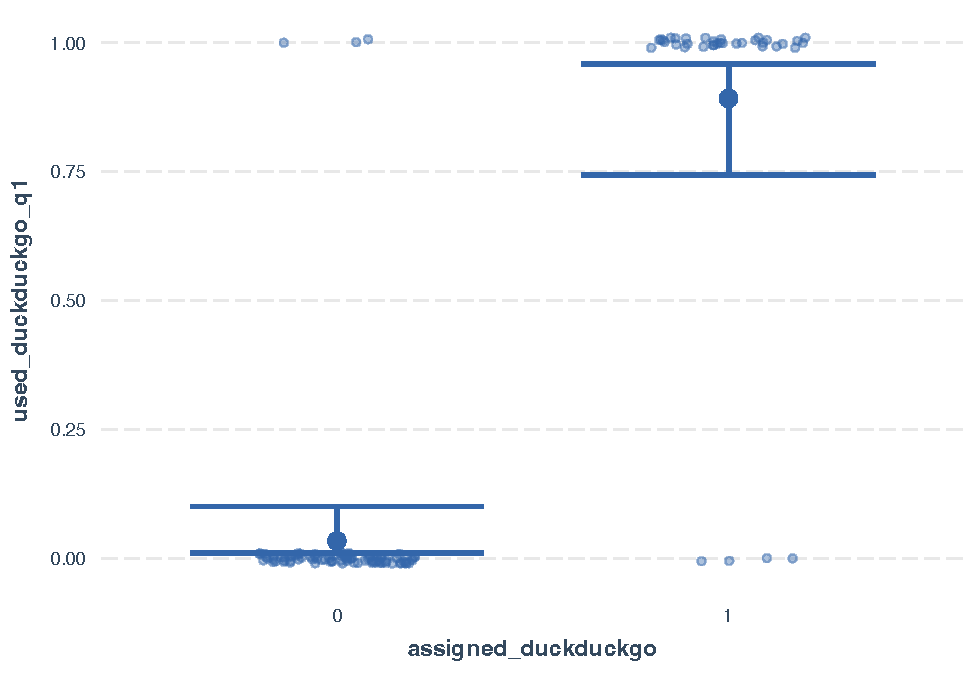
\includegraphics{analysis-July19_files/figure-latex/unnamed-chunk-22-1.pdf}

\begin{Shaded}
\begin{Highlighting}[]
\CommentTok{\# Check q3}

\NormalTok{sqdefddgq3 }\OtherTok{=} \FunctionTok{glm}\NormalTok{(used\_duckduckgo\_q3 }\SpecialCharTok{\textasciitilde{}}\NormalTok{ assigned\_duckduckgo, }\AttributeTok{data=}\NormalTok{dfexp\_def\_s, }\AttributeTok{family =}\StringTok{"binomial"}\NormalTok{)}

\NormalTok{plotsqdefddgq3 }\OtherTok{=} \FunctionTok{effect\_plot}\NormalTok{(sqdefddgq3, }\AttributeTok{pred =} \StringTok{"assigned\_duckduckgo"}\NormalTok{, }\AttributeTok{interval =} \ConstantTok{TRUE}\NormalTok{, }\AttributeTok{plot.points =} \ConstantTok{TRUE}\NormalTok{, }\AttributeTok{jitter =} \FunctionTok{c}\NormalTok{(}\FloatTok{0.2}\NormalTok{, }\FloatTok{0.01}\NormalTok{), }\AttributeTok{point.alpha =} \FloatTok{0.4}\NormalTok{, }\AttributeTok{colors =} \StringTok{"Qual1"}\NormalTok{)}

\NormalTok{plotsqdefddgq3}
\end{Highlighting}
\end{Shaded}

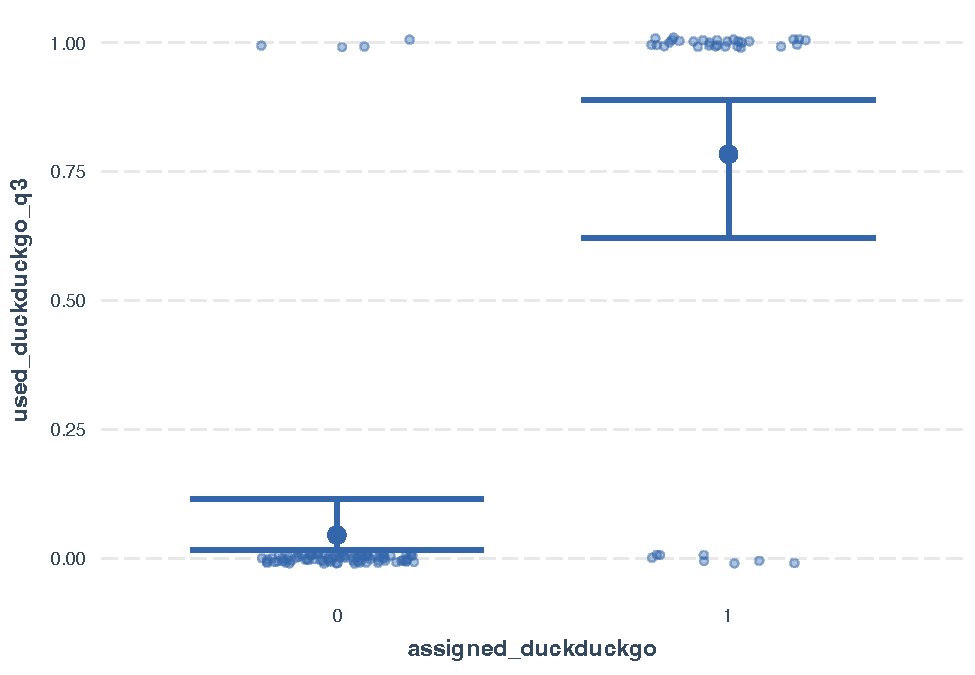
\includegraphics{analysis-July19_files/figure-latex/unnamed-chunk-22-2.pdf}

\begin{Shaded}
\begin{Highlighting}[]
\NormalTok{sqyahooq3}\OtherTok{=} \FunctionTok{glm}\NormalTok{(used\_yahoo\_q3 }\SpecialCharTok{\textasciitilde{}}\NormalTok{ forced\_choice\_s, }\AttributeTok{data=}\NormalTok{dfyahoo, }\AttributeTok{family =}\StringTok{"binomial"}\NormalTok{)}

\NormalTok{plotyahooq3 }\OtherTok{=} \FunctionTok{effect\_plot}\NormalTok{(sqyahooq3, }\AttributeTok{pred =} \StringTok{"forced\_choice\_s"}\NormalTok{, }\AttributeTok{interval =} \ConstantTok{TRUE}\NormalTok{, }\AttributeTok{plot.points =} \ConstantTok{TRUE}\NormalTok{, }\AttributeTok{jitter =} \FunctionTok{c}\NormalTok{(}\FloatTok{0.2}\NormalTok{, }\FloatTok{0.01}\NormalTok{), }\AttributeTok{point.alpha =} \FloatTok{0.4}\NormalTok{, }\AttributeTok{colors =} \StringTok{"Qual1"}\NormalTok{)}

\NormalTok{plotyahooq3}
\end{Highlighting}
\end{Shaded}

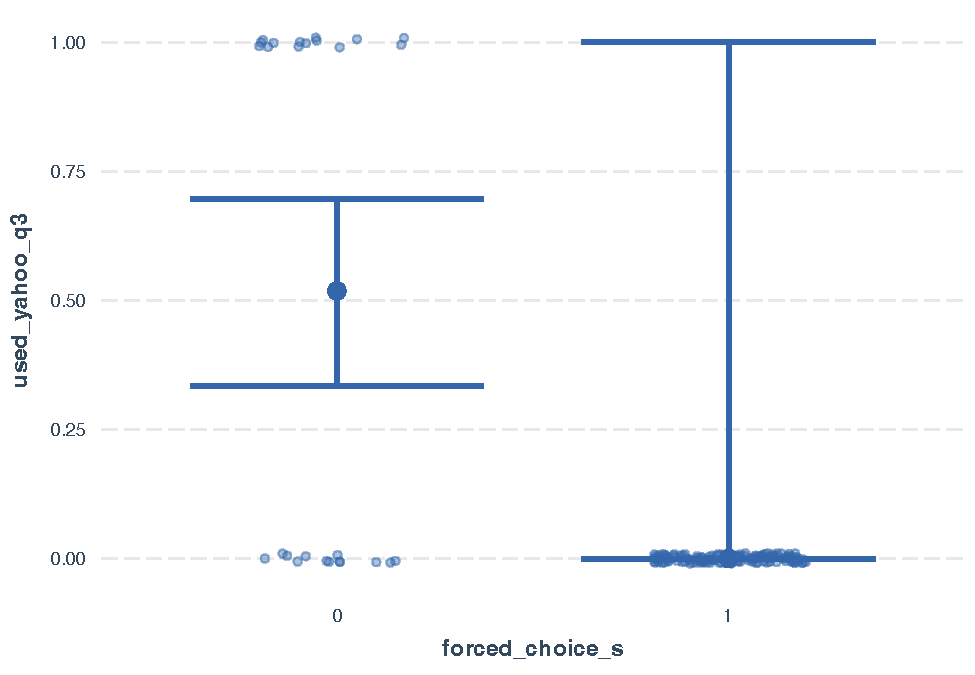
\includegraphics{analysis-July19_files/figure-latex/unnamed-chunk-23-1.pdf}
Compare with other defaults. Do chi-squared test.

\begin{Shaded}
\begin{Highlighting}[]
\NormalTok{yahooq1 }\OtherTok{=} \FunctionTok{glm}\NormalTok{(}\AttributeTok{data =}\NormalTok{ dfexp\_def\_s, used\_yahoo\_q1 }\SpecialCharTok{\textasciitilde{}}\NormalTok{ assigned\_yahoo }\SpecialCharTok{+}\NormalTok{ yahoo\_prior, }\AttributeTok{family =} \StringTok{"binomial"}\NormalTok{)}

\FunctionTok{summary}\NormalTok{(yahooq1)}
\end{Highlighting}
\end{Shaded}

\begin{verbatim}
## 
## Call:
## glm(formula = used_yahoo_q1 ~ assigned_yahoo + yahoo_prior, family = "binomial", 
##     data = dfexp_def_s)
## 
## Coefficients:
##                 Estimate Std. Error z value Pr(>|z|)
## (Intercept)      -21.897   2886.766  -0.008    0.994
## assigned_yahoo1   21.763   2886.766   0.008    0.994
## yahoo_prior        1.232      0.844   1.460    0.144
## 
## (Dispersion parameter for binomial family taken to be 1)
## 
##     Null deviance: 95.915  on 125  degrees of freedom
## Residual deviance: 34.224  on 123  degrees of freedom
## AIC: 40.224
## 
## Number of Fisher Scoring iterations: 20
\end{verbatim}

\begin{Shaded}
\begin{Highlighting}[]
\FunctionTok{lm}\NormalTok{(}\AttributeTok{data =}\NormalTok{ dfexp\_def\_s, used\_yahoo\_q1 }\SpecialCharTok{\textasciitilde{}}\NormalTok{ assigned\_yahoo }\SpecialCharTok{+}\NormalTok{ yahoo\_prior }\SpecialCharTok{+}\NormalTok{ yahoo\_qual)}
\end{Highlighting}
\end{Shaded}

\begin{verbatim}
## 
## Call:
## lm(formula = used_yahoo_q1 ~ assigned_yahoo + yahoo_prior + yahoo_qual, 
##     data = dfexp_def_s)
## 
## Coefficients:
##     (Intercept)  assigned_yahoo1      yahoo_prior       yahoo_qual  
##        -0.10781          0.56504          0.07431          0.03965
\end{verbatim}

\hypertarget{big-regression-general-analysis-status-quo-effect}{%
\subsection{Big regression general analysis status quo effect}\label{big-regression-general-analysis-status-quo-effect}}

There si something wrong with the default data set. Showing NAs in assigned to a

\begin{Shaded}
\begin{Highlighting}[]
\NormalTok{dfexp\_def\_s }\OtherTok{=}\NormalTok{ dfexp\_def\_s }\SpecialCharTok{\%\textgreater{}\%} 
  \FunctionTok{mutate}\NormalTok{(}\AttributeTok{statquo\_sq1 =} \FunctionTok{ifelse}\NormalTok{(assigned\_bing}\SpecialCharTok{==}\DecValTok{1} \SpecialCharTok{\&}\NormalTok{ used\_bing\_q1}\SpecialCharTok{==}\DecValTok{1} \SpecialCharTok{|}\NormalTok{ assigned\_google}\SpecialCharTok{==}\DecValTok{1} \SpecialCharTok{\&}\NormalTok{ used\_google\_q1}\SpecialCharTok{==}\DecValTok{1} \SpecialCharTok{|}\NormalTok{ assigned\_duckduckgo}\SpecialCharTok{==}\DecValTok{1} \SpecialCharTok{\&}\NormalTok{ used\_duckduckgo\_q1}\SpecialCharTok{==}\DecValTok{1} \SpecialCharTok{|}\NormalTok{ assigned\_yahoo}\SpecialCharTok{==}\DecValTok{1} \SpecialCharTok{\&}\NormalTok{ used\_yahoo\_q1}\SpecialCharTok{==}\DecValTok{1}\NormalTok{, }\DecValTok{1}\NormalTok{, }\DecValTok{0}\NormalTok{),}
         \AttributeTok{statquo\_sq3=} \FunctionTok{ifelse}\NormalTok{(assigned\_bing}\SpecialCharTok{==}\DecValTok{1} \SpecialCharTok{\&}\NormalTok{ used\_bing\_q3}\SpecialCharTok{==}\DecValTok{1} \SpecialCharTok{|}\NormalTok{ assigned\_google}\SpecialCharTok{==}\DecValTok{1} \SpecialCharTok{\&}\NormalTok{ used\_google\_q3}\SpecialCharTok{==}\DecValTok{1}\SpecialCharTok{|}\NormalTok{assigned\_duckduckgo}\SpecialCharTok{==}\DecValTok{1} \SpecialCharTok{\&}\NormalTok{ used\_duckduckgo\_q3}\SpecialCharTok{==}\DecValTok{1} \SpecialCharTok{|}\NormalTok{ assigned\_yahoo}\SpecialCharTok{==}\DecValTok{1} \SpecialCharTok{\&}\NormalTok{ used\_yahoo\_q3}\SpecialCharTok{==}\DecValTok{1}\NormalTok{, }\DecValTok{1}\NormalTok{, }\DecValTok{0}\NormalTok{),}
         \AttributeTok{prior\_use =} \FunctionTok{ifelse}\NormalTok{(assigned\_google}\SpecialCharTok{==}\DecValTok{1} \SpecialCharTok{\&}\NormalTok{ google\_prior}\SpecialCharTok{==}\DecValTok{1} \SpecialCharTok{|}\NormalTok{ assigned\_bing}\SpecialCharTok{==}\DecValTok{1} \SpecialCharTok{\&}\NormalTok{ bing\_prior}\SpecialCharTok{==}\DecValTok{1} \SpecialCharTok{|}\NormalTok{ assigned\_duckduckgo}\SpecialCharTok{==}\DecValTok{1} \SpecialCharTok{\&}\NormalTok{ ddg\_pior}\SpecialCharTok{==}\DecValTok{1} \SpecialCharTok{|}\NormalTok{ assigned\_yahoo}\SpecialCharTok{==}\DecValTok{1} \SpecialCharTok{\&}\NormalTok{ yahoo\_prior}\SpecialCharTok{==}\DecValTok{1}\NormalTok{,}\DecValTok{1}\NormalTok{,}\DecValTok{0}\NormalTok{),}
         \AttributeTok{explor\_sq1 =} \FunctionTok{ifelse}\NormalTok{(}\FunctionTok{str\_length}\NormalTok{(se\_beatles)}\SpecialCharTok{\textgreater{}}\DecValTok{1}\NormalTok{, }\DecValTok{1}\NormalTok{,}\DecValTok{0}\NormalTok{),}
         \AttributeTok{age =} \DecValTok{2023} \SpecialCharTok{{-}} \FunctionTok{as.numeric}\NormalTok{(q32),}
         \AttributeTok{age\_c =} \FunctionTok{case\_when}\NormalTok{(age}\SpecialCharTok{\textless{}}\DecValTok{30} \SpecialCharTok{\textasciitilde{}} \StringTok{"18{-}29"}\NormalTok{,}
\NormalTok{                           age }\SpecialCharTok{\textgreater{}}\DecValTok{29} \SpecialCharTok{\&}\NormalTok{ age }\SpecialCharTok{\textless{}}\DecValTok{40} \SpecialCharTok{\textasciitilde{}} \StringTok{"30{-}39"}\NormalTok{,}
\NormalTok{                           age }\SpecialCharTok{\textgreater{}}\DecValTok{39} \SpecialCharTok{\&}\NormalTok{ age }\SpecialCharTok{\textless{}}\DecValTok{50} \SpecialCharTok{\textasciitilde{}} \StringTok{"40{-}49"}\NormalTok{,}
\NormalTok{                           age}\SpecialCharTok{\textgreater{}}\DecValTok{49} \SpecialCharTok{\&}\NormalTok{ age }\SpecialCharTok{\textless{}}\DecValTok{60} \SpecialCharTok{\textasciitilde{}} \StringTok{"50{-}59"}\NormalTok{,}
\NormalTok{                           age}\SpecialCharTok{\textgreater{}}\DecValTok{59} \SpecialCharTok{\textasciitilde{}} \StringTok{"60 +"}\NormalTok{))}


\FunctionTok{lm}\NormalTok{(}\AttributeTok{data=}\NormalTok{dfexp\_def\_s, }\AttributeTok{formula=}\NormalTok{ statquo\_sq1 }\SpecialCharTok{\textasciitilde{}}\NormalTok{  prior\_use)}
\end{Highlighting}
\end{Shaded}

\begin{verbatim}
## 
## Call:
## lm(formula = statquo_sq1 ~ prior_use, data = dfexp_def_s)
## 
## Coefficients:
## (Intercept)    prior_use  
##      0.6000       0.3186
\end{verbatim}

\begin{Shaded}
\begin{Highlighting}[]
\FunctionTok{lm}\NormalTok{(}\AttributeTok{data=}\NormalTok{dfexp\_def\_s, }\AttributeTok{formula=}\NormalTok{ statquo\_sq1 }\SpecialCharTok{\textasciitilde{}}\NormalTok{ prior\_use }\SpecialCharTok{+}\NormalTok{ age\_c)}
\end{Highlighting}
\end{Shaded}

\begin{verbatim}
## 
## Call:
## lm(formula = statquo_sq1 ~ prior_use + age_c, data = dfexp_def_s)
## 
## Coefficients:
## (Intercept)    prior_use   age_c30-39   age_c40-49   age_c50-59    age_c60 +  
##     0.64683      0.31029     -0.05514     -0.02280     -0.08007     -0.10985
\end{verbatim}

Data defaults without Google

\begin{Shaded}
\begin{Highlighting}[]
\NormalTok{dfexp\_def\_s2 }\OtherTok{=}\NormalTok{ dfexp\_def\_s }\SpecialCharTok{\%\textgreater{}\%} 
  \FunctionTok{filter}\NormalTok{(assigned\_google}\SpecialCharTok{==}\DecValTok{0}\NormalTok{)}
\end{Highlighting}
\end{Shaded}

\begin{Shaded}
\begin{Highlighting}[]
\FunctionTok{lm}\NormalTok{(}\AttributeTok{data=}\NormalTok{dfexp\_def\_s2, }\AttributeTok{formula=}\NormalTok{ statquo\_sq1 }\SpecialCharTok{\textasciitilde{}}\NormalTok{ explor\_sq1 }\SpecialCharTok{+}\NormalTok{ prior\_use)}
\end{Highlighting}
\end{Shaded}

\begin{verbatim}
## 
## Call:
## lm(formula = statquo_sq1 ~ explor_sq1 + prior_use, data = dfexp_def_s2)
## 
## Coefficients:
## (Intercept)   explor_sq1    prior_use  
##      0.6154       0.1091       0.2755
\end{verbatim}

\begin{Shaded}
\begin{Highlighting}[]
\NormalTok{glmsqs1 }\OtherTok{=} \FunctionTok{glm}\NormalTok{(}\AttributeTok{data=}\NormalTok{dfexp\_def\_s2, }\AttributeTok{formula=}\NormalTok{ statquo\_sq1 }\SpecialCharTok{\textasciitilde{}}\NormalTok{ explor\_sq1 }\SpecialCharTok{+}\NormalTok{ prior\_use, }\AttributeTok{family =} \StringTok{"binomial"}\NormalTok{)}

\FunctionTok{summary}\NormalTok{(glmsqs1)}
\end{Highlighting}
\end{Shaded}

\begin{verbatim}
## 
## Call:
## glm(formula = statquo_sq1 ~ explor_sq1 + prior_use, family = "binomial", 
##     data = dfexp_def_s2)
## 
## Coefficients:
##              Estimate Std. Error z value Pr(>|z|)   
## (Intercept)    0.4700     0.3291   1.428  0.15330   
## explor_sq1    13.4660  1455.3976   0.009  0.99262   
## prior_use      1.6301     0.5435   2.999  0.00271 **
## ---
## Signif. codes:  0 '***' 0.001 '**' 0.01 '*' 0.05 '.' 0.1 ' ' 1
## 
## (Dispersion parameter for binomial family taken to be 1)
## 
##     Null deviance: 100.365  on 94  degrees of freedom
## Residual deviance:  89.877  on 92  degrees of freedom
## AIC: 95.877
## 
## Number of Fisher Scoring iterations: 14
\end{verbatim}

Interesting coefficients, qualitatively. Now, run glm because p\textgreater1

\begin{Shaded}
\begin{Highlighting}[]
\FunctionTok{mean}\NormalTok{(dfexp\_def\_s}\SpecialCharTok{$}\NormalTok{statquo\_sq1) }
\end{Highlighting}
\end{Shaded}

\begin{verbatim}
## [1] 0.8174603
\end{verbatim}

\hypertarget{check-if-those-who-use-the-default-use-another-one-too}{%
\subsection{Check if those who use the default use another one too!}\label{check-if-those-who-use-the-default-use-another-one-too}}

This is important. q1 only a few use more than one, q3 many more explore.

\begin{Shaded}
\begin{Highlighting}[]
\CommentTok{\# Create var for analysis}

\NormalTok{dfexp\_def\_s }\OtherTok{=}\NormalTok{ dfexp\_def\_s }\SpecialCharTok{\%\textgreater{}\%} 
  \FunctionTok{mutate}\NormalTok{(}\AttributeTok{se\_assigned =} \FunctionTok{case\_when}\NormalTok{(assigned\_google}\SpecialCharTok{==}\DecValTok{1} \SpecialCharTok{\textasciitilde{}} \StringTok{"Google"}\NormalTok{,}
\NormalTok{                                 assigned\_bing}\SpecialCharTok{==}\DecValTok{1} \SpecialCharTok{\textasciitilde{}} \StringTok{"Bing"}\NormalTok{,}
\NormalTok{                                 assigned\_duckduckgo}\SpecialCharTok{==}\DecValTok{1} \SpecialCharTok{\textasciitilde{}}\StringTok{"DuckDuck Go"}\NormalTok{,}
\NormalTok{                                 assigned\_yahoo}\SpecialCharTok{==}\DecValTok{1} \SpecialCharTok{\textasciitilde{}} \StringTok{"Yahoo"}\NormalTok{))}
\end{Highlighting}
\end{Shaded}

Code below irrelevant. q1 only one person used more than one

\begin{Shaded}
\begin{Highlighting}[]
\CommentTok{\# glm\_just\_one= glm(just\_one\_sq1 \textasciitilde{} se\_assigned, data=dfexp\_def\_s, family ="binomial")}
\CommentTok{\# }
\CommentTok{\# plot\_just\_one\_sq1 = effect\_plot(glm\_just\_one, pred = "se\_assigned", interval = TRUE, plot.points = TRUE, jitter = c(0.2, 0.01), point.alpha = 0.4, colors = "Qual1")}
\CommentTok{\# }
\CommentTok{\# plot\_just\_one\_sq1}

\FunctionTok{table}\NormalTok{(dfexp\_def\_s}\SpecialCharTok{$}\NormalTok{se\_assigned, dfexp\_def\_s}\SpecialCharTok{$}\NormalTok{just\_one\_sq1)}
\end{Highlighting}
\end{Shaded}

\begin{verbatim}
##              
##                0  1
##   Bing         1 30
##   DuckDuck Go  0 37
##   Google       0 31
##   Yahoo        0 27
\end{verbatim}

\begin{Shaded}
\begin{Highlighting}[]
\FunctionTok{table}\NormalTok{(dfexp\_def\_s}\SpecialCharTok{$}\NormalTok{se\_assigned, dfexp\_def\_s}\SpecialCharTok{$}\NormalTok{just\_one\_sq2)}
\end{Highlighting}
\end{Shaded}

\begin{verbatim}
##              
##                0  1
##   Bing         4 27
##   DuckDuck Go  1 36
##   Google       1 30
##   Yahoo        2 25
\end{verbatim}

\begin{Shaded}
\begin{Highlighting}[]
\FunctionTok{table}\NormalTok{(dfexp\_def\_s}\SpecialCharTok{$}\NormalTok{se\_assigned, dfexp\_def\_s}\SpecialCharTok{$}\NormalTok{just\_one\_sq3)}
\end{Highlighting}
\end{Shaded}

\begin{verbatim}
##              
##                0  1
##   Bing         2 29
##   DuckDuck Go  2 35
##   Google       0 31
##   Yahoo        1 26
\end{verbatim}

Code above is not what I need. The relevant variable is stat\_quo\_qi * just\_one\_qi

\begin{Shaded}
\begin{Highlighting}[]
\NormalTok{dfexp\_def\_s }\OtherTok{=}\NormalTok{ dfexp\_def\_s }\SpecialCharTok{\%\textgreater{}\%} 
  \FunctionTok{mutate}\NormalTok{(}\AttributeTok{just\_default\_sq1 =} \FunctionTok{ifelse}\NormalTok{(statquo\_sq1}\SpecialCharTok{==}\DecValTok{1} \SpecialCharTok{\&}\NormalTok{ just\_one\_sq1}\SpecialCharTok{==}\DecValTok{1}\NormalTok{,}\DecValTok{1}\NormalTok{,}\DecValTok{0}\NormalTok{),}
         \AttributeTok{just\_default\_sq3 =} \FunctionTok{ifelse}\NormalTok{(statquo\_sq3}\SpecialCharTok{==}\DecValTok{1} \SpecialCharTok{\&}\NormalTok{ just\_one\_sq3}\SpecialCharTok{==}\DecValTok{1}\NormalTok{,}\DecValTok{1}\NormalTok{,}\DecValTok{0}\NormalTok{))}
\end{Highlighting}
\end{Shaded}

\begin{Shaded}
\begin{Highlighting}[]
\FunctionTok{table}\NormalTok{(dfexp\_def\_s}\SpecialCharTok{$}\NormalTok{se\_assigned, dfexp\_def\_s}\SpecialCharTok{$}\NormalTok{just\_default\_sq1)}
\end{Highlighting}
\end{Shaded}

\begin{verbatim}
##              
##                0  1
##   Bing         7 24
##   DuckDuck Go  4 33
##   Google       2 29
##   Yahoo       11 16
\end{verbatim}

\begin{Shaded}
\begin{Highlighting}[]
\FunctionTok{table}\NormalTok{(dfexp\_def\_s}\SpecialCharTok{$}\NormalTok{se\_assigned, dfexp\_def\_s}\SpecialCharTok{$}\NormalTok{just\_default\_sq3)}
\end{Highlighting}
\end{Shaded}

\begin{verbatim}
##              
##                0  1
##   Bing        11 20
##   DuckDuck Go 10 27
##   Google       2 29
##   Yahoo       14 13
\end{verbatim}

\hypertarget{now-with-the-second-experiment}{%
\subsubsection{Now with the second experiment}\label{now-with-the-second-experiment}}

\begin{Shaded}
\begin{Highlighting}[]
\NormalTok{datexp }\OtherTok{=}\NormalTok{ datexp }\SpecialCharTok{\%\textgreater{}\%} 
  \FunctionTok{mutate}\NormalTok{(}\AttributeTok{se\_assigned =} \FunctionTok{case\_when}\NormalTok{(assigned\_google}\SpecialCharTok{==}\DecValTok{1} \SpecialCharTok{\textasciitilde{}} \StringTok{"Google"}\NormalTok{,}
\NormalTok{                                 assigned\_bing}\SpecialCharTok{==}\DecValTok{1} \SpecialCharTok{\textasciitilde{}} \StringTok{"Bing"}\NormalTok{),}
         \AttributeTok{statquo\_sq1 =} \FunctionTok{ifelse}\NormalTok{(assigned\_bing}\SpecialCharTok{==}\DecValTok{1} \SpecialCharTok{\&}\NormalTok{ used\_bing\_q1}\SpecialCharTok{==}\DecValTok{1} \SpecialCharTok{|}\NormalTok{ assigned\_google}\SpecialCharTok{==}\DecValTok{1} \SpecialCharTok{\&}\NormalTok{ used\_google\_q1}\SpecialCharTok{==}\DecValTok{1}\NormalTok{, }\DecValTok{1}\NormalTok{, }\DecValTok{0}\NormalTok{),}
         \AttributeTok{statquo\_sq2 =} \FunctionTok{ifelse}\NormalTok{(assigned\_bing}\SpecialCharTok{==}\DecValTok{1} \SpecialCharTok{\&}\NormalTok{ used\_bing\_q2}\SpecialCharTok{==}\DecValTok{1} \SpecialCharTok{|}\NormalTok{ assigned\_google}\SpecialCharTok{==}\DecValTok{1} \SpecialCharTok{\&}\NormalTok{ used\_google\_q2}\SpecialCharTok{==}\DecValTok{1}\NormalTok{, }\DecValTok{1}\NormalTok{, }\DecValTok{0}\NormalTok{),}
         \AttributeTok{statquo\_sq3=} \FunctionTok{ifelse}\NormalTok{(assigned\_bing}\SpecialCharTok{==}\DecValTok{1} \SpecialCharTok{\&}\NormalTok{ used\_bing\_q3}\SpecialCharTok{==}\DecValTok{1} \SpecialCharTok{|}\NormalTok{ assigned\_google}\SpecialCharTok{==}\DecValTok{1} \SpecialCharTok{\&}\NormalTok{ used\_google\_q3}\SpecialCharTok{==}\DecValTok{1}\NormalTok{, }\DecValTok{1}\NormalTok{, }\DecValTok{0}\NormalTok{),}
         \AttributeTok{statquo\_sq4 =} \FunctionTok{ifelse}\NormalTok{(assigned\_bing}\SpecialCharTok{==}\DecValTok{1} \SpecialCharTok{\&}\NormalTok{ used\_bing\_q4}\SpecialCharTok{==}\DecValTok{1} \SpecialCharTok{|}\NormalTok{ assigned\_google}\SpecialCharTok{==}\DecValTok{1} \SpecialCharTok{\&}\NormalTok{ used\_google\_q4}\SpecialCharTok{==}\DecValTok{1}\NormalTok{, }\DecValTok{1}\NormalTok{, }\DecValTok{0}\NormalTok{),}
         \AttributeTok{statquo\_sq5 =} \FunctionTok{ifelse}\NormalTok{(assigned\_bing}\SpecialCharTok{==}\DecValTok{1} \SpecialCharTok{\&}\NormalTok{ used\_bing\_q5}\SpecialCharTok{==}\DecValTok{1} \SpecialCharTok{|}\NormalTok{ assigned\_google}\SpecialCharTok{==}\DecValTok{1} \SpecialCharTok{\&}\NormalTok{ used\_google\_q5}\SpecialCharTok{==}\DecValTok{1}\NormalTok{, }\DecValTok{1}\NormalTok{, }\DecValTok{0}\NormalTok{),}
         \AttributeTok{prior\_use =} \FunctionTok{ifelse}\NormalTok{(assigned\_google}\SpecialCharTok{==}\DecValTok{1} \SpecialCharTok{\&}\NormalTok{ google\_prior}\SpecialCharTok{==}\DecValTok{1} \SpecialCharTok{|}\NormalTok{ assigned\_bing}\SpecialCharTok{==}\DecValTok{1} \SpecialCharTok{\&}\NormalTok{ bing\_prior}\SpecialCharTok{==}\DecValTok{1}\NormalTok{,}\DecValTok{1}\NormalTok{,}\DecValTok{0}\NormalTok{),}
         \AttributeTok{just\_default\_sq1 =} \FunctionTok{ifelse}\NormalTok{(statquo\_sq1}\SpecialCharTok{==}\DecValTok{1} \SpecialCharTok{\&}\NormalTok{ just\_one\_sq1}\SpecialCharTok{==}\DecValTok{1}\NormalTok{,}\DecValTok{1}\NormalTok{,}\DecValTok{0}\NormalTok{),}
         \AttributeTok{just\_default\_sq2 =} \FunctionTok{ifelse}\NormalTok{(statquo\_sq2}\SpecialCharTok{==}\DecValTok{1} \SpecialCharTok{\&}\NormalTok{ just\_one\_sq3}\SpecialCharTok{==}\DecValTok{1}\NormalTok{,}\DecValTok{1}\NormalTok{,}\DecValTok{0}\NormalTok{),}
         \AttributeTok{just\_default\_sq3 =} \FunctionTok{ifelse}\NormalTok{(statquo\_sq3}\SpecialCharTok{==}\DecValTok{1} \SpecialCharTok{\&}\NormalTok{ just\_one\_sq3}\SpecialCharTok{==}\DecValTok{1}\NormalTok{,}\DecValTok{1}\NormalTok{,}\DecValTok{0}\NormalTok{),}
         \AttributeTok{just\_default\_sq4 =} \FunctionTok{ifelse}\NormalTok{(statquo\_sq4}\SpecialCharTok{==}\DecValTok{1} \SpecialCharTok{\&}\NormalTok{ just\_one\_sq3}\SpecialCharTok{==}\DecValTok{1}\NormalTok{,}\DecValTok{1}\NormalTok{,}\DecValTok{0}\NormalTok{),}
         \AttributeTok{just\_default\_sq5 =} \FunctionTok{ifelse}\NormalTok{(statquo\_sq5}\SpecialCharTok{==}\DecValTok{1} \SpecialCharTok{\&}\NormalTok{ just\_one\_sq3}\SpecialCharTok{==}\DecValTok{1}\NormalTok{,}\DecValTok{1}\NormalTok{,}\DecValTok{0}\NormalTok{))}
\end{Highlighting}
\end{Shaded}

\begin{Shaded}
\begin{Highlighting}[]
\FunctionTok{table}\NormalTok{(datexp}\SpecialCharTok{$}\NormalTok{se\_assigned, datexp}\SpecialCharTok{$}\NormalTok{just\_default\_sq1)}
\end{Highlighting}
\end{Shaded}

\begin{verbatim}
##         
##            0   1
##   Bing    45 112
##   Google   9 153
\end{verbatim}

\begin{Shaded}
\begin{Highlighting}[]
\FunctionTok{table}\NormalTok{(datexp}\SpecialCharTok{$}\NormalTok{se\_assigned, datexp}\SpecialCharTok{$}\NormalTok{just\_default\_sq2)}
\end{Highlighting}
\end{Shaded}

\begin{verbatim}
##         
##            0   1
##   Bing    67  90
##   Google  12 150
\end{verbatim}

\begin{Shaded}
\begin{Highlighting}[]
\FunctionTok{table}\NormalTok{(datexp}\SpecialCharTok{$}\NormalTok{se\_assigned, datexp}\SpecialCharTok{$}\NormalTok{just\_default\_sq3)}
\end{Highlighting}
\end{Shaded}

\begin{verbatim}
##         
##            0   1
##   Bing    78  79
##   Google   9 153
\end{verbatim}

\begin{Shaded}
\begin{Highlighting}[]
\FunctionTok{table}\NormalTok{(datexp}\SpecialCharTok{$}\NormalTok{se\_assigned, datexp}\SpecialCharTok{$}\NormalTok{just\_default\_sq4)}
\end{Highlighting}
\end{Shaded}

\begin{verbatim}
##         
##            0   1
##   Bing    82  75
##   Google  12 150
\end{verbatim}

\begin{Shaded}
\begin{Highlighting}[]
\FunctionTok{table}\NormalTok{(datexp}\SpecialCharTok{$}\NormalTok{se\_assigned, datexp}\SpecialCharTok{$}\NormalTok{just\_default\_sq5)}
\end{Highlighting}
\end{Shaded}

\begin{verbatim}
##         
##            0   1
##   Bing    84  73
##   Google  18 144
\end{verbatim}

Interesting result. More people tend to use Bing exclusively over time.

\hypertarget{results-weather-apps}{%
\section{Results Weather Apps}\label{results-weather-apps}}

\begin{Shaded}
\begin{Highlighting}[]
\CommentTok{\# The same for weather apps part}

\NormalTok{dfexp2 }\OtherTok{=}\NormalTok{ dfexp }\SpecialCharTok{\%\textgreater{}\%} 
  \FunctionTok{mutate}\NormalTok{(}\AttributeTok{chose\_wc =} \FunctionTok{if\_else}\NormalTok{(choice\_screen\_2 }\SpecialCharTok{==} \DecValTok{1}\NormalTok{, }\DecValTok{1}\NormalTok{, }\DecValTok{0}\NormalTok{, }\ConstantTok{NULL}\NormalTok{),}
         \AttributeTok{chose\_aw =} \FunctionTok{if\_else}\NormalTok{(choice\_screen\_2 }\SpecialCharTok{==} \DecValTok{2}\NormalTok{,}\DecValTok{1}\NormalTok{,}\DecValTok{0}\NormalTok{, }\ConstantTok{NULL}\NormalTok{),}
         \AttributeTok{chose\_wu =} \FunctionTok{if\_else}\NormalTok{(choice\_screen\_2 }\SpecialCharTok{==} \DecValTok{3}\NormalTok{, }\DecValTok{1}\NormalTok{,}\DecValTok{0}\NormalTok{, }\ConstantTok{NULL}\NormalTok{),}
         
         \AttributeTok{choice\_wa =} \FunctionTok{factor}\NormalTok{(}\FunctionTok{case\_when}\NormalTok{(chose\_wc }\SpecialCharTok{==} \DecValTok{1} \SpecialCharTok{\textasciitilde{}} \StringTok{"Weather Channel"}\NormalTok{,}
\NormalTok{                            chose\_aw }\SpecialCharTok{==} \DecValTok{1} \SpecialCharTok{\textasciitilde{}} \StringTok{"AccuWeather"}\NormalTok{,}
\NormalTok{                            chose\_wu }\SpecialCharTok{==} \DecValTok{1} \SpecialCharTok{\textasciitilde{}} \StringTok{"Weather Underground"}\NormalTok{),}
                         \AttributeTok{levels =} \FunctionTok{c}\NormalTok{(}\StringTok{"Weather Channel"}\NormalTok{, }
                                    \StringTok{"AccuWeather"}\NormalTok{, }
                                    \StringTok{"WeatherUnderground"}\NormalTok{)),}
         
         \AttributeTok{assigned\_wc =} \FunctionTok{ifelse}\NormalTok{(weather\_do }\SpecialCharTok{\%in\%} \StringTok{"default\_wc"}\NormalTok{, }\DecValTok{1}\NormalTok{, }\DecValTok{0}\NormalTok{), }
         \AttributeTok{assigned\_aw =} \FunctionTok{ifelse}\NormalTok{(weather\_do }\SpecialCharTok{\%in\%} \StringTok{"default\_aw"}\NormalTok{, }\DecValTok{1}\NormalTok{, }\DecValTok{0}\NormalTok{),}
         \AttributeTok{assigned\_wu =} \FunctionTok{ifelse}\NormalTok{(weather\_do }\SpecialCharTok{\%in\%} \StringTok{"default\_wu"}\NormalTok{, }\DecValTok{1}\NormalTok{, }\DecValTok{0}\NormalTok{),}
         
         \AttributeTok{used\_wc\_q1 =} \FunctionTok{if\_else}\NormalTok{(}\FunctionTok{grepl}\NormalTok{(}\StringTok{"1"}\NormalTok{, app\_austin), }\DecValTok{1}\NormalTok{, }\DecValTok{0}\NormalTok{, }\ConstantTok{NULL}\NormalTok{),}
         \AttributeTok{used\_aw\_q1 =} \FunctionTok{if\_else}\NormalTok{(}\FunctionTok{grepl}\NormalTok{(}\StringTok{"2"}\NormalTok{, app\_austin),}\DecValTok{1}\NormalTok{,}\DecValTok{0}\NormalTok{,}\ConstantTok{NULL}\NormalTok{),}
         \AttributeTok{used\_wu\_q1 =} \FunctionTok{if\_else}\NormalTok{(}\FunctionTok{grepl}\NormalTok{(}\StringTok{"3"}\NormalTok{, app\_austin),}\DecValTok{1}\NormalTok{,}\DecValTok{0}\NormalTok{,}\ConstantTok{NULL}\NormalTok{),}
         \AttributeTok{used\_other\_q1 =} \FunctionTok{if\_else}\NormalTok{(}\FunctionTok{grepl}\NormalTok{(}\StringTok{"4"}\NormalTok{, app\_austin),}\DecValTok{1}\NormalTok{,}\DecValTok{0}\NormalTok{,}\ConstantTok{NULL}\NormalTok{),}
         
         \AttributeTok{used\_wc\_q2 =} \FunctionTok{if\_else}\NormalTok{(}\FunctionTok{grepl}\NormalTok{(}\StringTok{"1"}\NormalTok{, app\_cambridge), }\DecValTok{1}\NormalTok{, }\DecValTok{0}\NormalTok{, }\ConstantTok{NULL}\NormalTok{),}
         \AttributeTok{used\_aw\_q2 =} \FunctionTok{if\_else}\NormalTok{(}\FunctionTok{grepl}\NormalTok{(}\StringTok{"2"}\NormalTok{, app\_cambridge),}\DecValTok{1}\NormalTok{,}\DecValTok{0}\NormalTok{,}\ConstantTok{NULL}\NormalTok{),}
         \AttributeTok{used\_wu\_q2 =} \FunctionTok{if\_else}\NormalTok{(}\FunctionTok{grepl}\NormalTok{(}\StringTok{"3"}\NormalTok{, app\_cambridge),}\DecValTok{1}\NormalTok{,}\DecValTok{0}\NormalTok{,}\ConstantTok{NULL}\NormalTok{),}
         
         \AttributeTok{used\_wc\_q3 =} \FunctionTok{if\_else}\NormalTok{(}\FunctionTok{grepl}\NormalTok{(}\StringTok{"1"}\NormalTok{, app\_cupertino), }\DecValTok{1}\NormalTok{, }\DecValTok{0}\NormalTok{, }\ConstantTok{NULL}\NormalTok{),}
         \AttributeTok{used\_aw\_q3 =} \FunctionTok{if\_else}\NormalTok{(}\FunctionTok{grepl}\NormalTok{(}\StringTok{"2"}\NormalTok{, app\_cupertino),}\DecValTok{1}\NormalTok{,}\DecValTok{0}\NormalTok{,}\ConstantTok{NULL}\NormalTok{),}
         \AttributeTok{used\_wu\_q3 =} \FunctionTok{if\_else}\NormalTok{(}\FunctionTok{grepl}\NormalTok{(}\StringTok{"3"}\NormalTok{, app\_cupertino),}\DecValTok{1}\NormalTok{,}\DecValTok{0}\NormalTok{,}\ConstantTok{NULL}\NormalTok{),}

         \AttributeTok{ac\_qual =}\NormalTok{ q31\_1,}
         \AttributeTok{aw\_qual =}\NormalTok{ q31\_2,}
         \AttributeTok{wu\_qual =}\NormalTok{ q31\_3,}
         
         \AttributeTok{ac\_prior =} \FunctionTok{ifelse}\NormalTok{(}\FunctionTok{grepl}\NormalTok{(}\StringTok{"1"}\NormalTok{, q54), }\DecValTok{1}\NormalTok{, }\DecValTok{0}\NormalTok{),}
         \AttributeTok{aw\_pior =} \FunctionTok{ifelse}\NormalTok{(}\FunctionTok{grepl}\NormalTok{(}\StringTok{"2"}\NormalTok{, q54),}\DecValTok{1}\NormalTok{, }\DecValTok{0}\NormalTok{),}
         \AttributeTok{wu\_prior =} \FunctionTok{ifelse}\NormalTok{(}\FunctionTok{grepl}\NormalTok{(}\StringTok{"3"}\NormalTok{, q54), }\DecValTok{1}\NormalTok{, }\DecValTok{0}\NormalTok{),}
         \AttributeTok{other\_prior =} \FunctionTok{ifelse}\NormalTok{(}\FunctionTok{grepl}\NormalTok{(}\StringTok{"4"}\NormalTok{, q54), }\DecValTok{1}\NormalTok{, }\DecValTok{0}\NormalTok{))}
\end{Highlighting}
\end{Shaded}

\begin{Shaded}
\begin{Highlighting}[]
\NormalTok{dfaw }\OtherTok{=}\NormalTok{ dfexp2 }\SpecialCharTok{\%\textgreater{}\%} 
  \FunctionTok{filter}\NormalTok{(forced\_choice\_w}\SpecialCharTok{==}\DecValTok{1}\SpecialCharTok{|}\NormalTok{ assigned\_aw}\SpecialCharTok{==}\DecValTok{1}\NormalTok{) }
\end{Highlighting}
\end{Shaded}

One plot for sq q1 for each (a1\_q1, a2\_q1, a3\_q1)

Another for sq q3 for each (a1\_q3, a2\_q3, a3\_q3)

\begin{Shaded}
\begin{Highlighting}[]
\CommentTok{\#AccuWeather}
\NormalTok{sqawq1}\OtherTok{=} \FunctionTok{glm}\NormalTok{(used\_aw\_q1 }\SpecialCharTok{\textasciitilde{}}\NormalTok{ forced\_choice\_w, }\AttributeTok{data=}\NormalTok{dfaw, }\AttributeTok{family =}\StringTok{"binomial"}\NormalTok{)}

\NormalTok{plotawq1 }\OtherTok{=} \FunctionTok{effect\_plot}\NormalTok{(sqawq1, }\AttributeTok{pred =} \StringTok{"forced\_choice\_w"}\NormalTok{, }\AttributeTok{interval =} \ConstantTok{TRUE}\NormalTok{, }\AttributeTok{plot.points =} \ConstantTok{TRUE}\NormalTok{, }\AttributeTok{jitter =} \FunctionTok{c}\NormalTok{(}\FloatTok{0.2}\NormalTok{, }\FloatTok{0.01}\NormalTok{), }\AttributeTok{point.alpha =} \FloatTok{0.4}\NormalTok{, }\AttributeTok{colors =} \StringTok{"Qual1"}\NormalTok{)}

\NormalTok{plotawq1}
\end{Highlighting}
\end{Shaded}

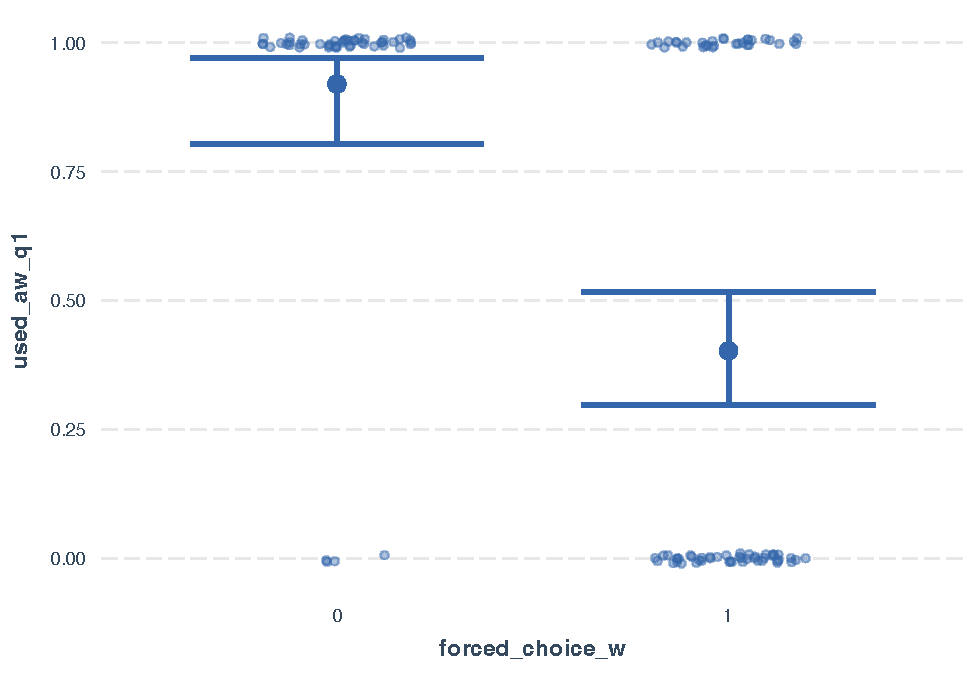
\includegraphics{analysis-July19_files/figure-latex/unnamed-chunk-37-1.pdf}

\begin{Shaded}
\begin{Highlighting}[]
\NormalTok{sqawq3}\OtherTok{=} \FunctionTok{glm}\NormalTok{(used\_aw\_q3 }\SpecialCharTok{\textasciitilde{}}\NormalTok{ forced\_choice\_w, }\AttributeTok{data=}\NormalTok{dfaw, }\AttributeTok{family =}\StringTok{"binomial"}\NormalTok{)}

\NormalTok{plotawq3 }\OtherTok{=} \FunctionTok{effect\_plot}\NormalTok{(sqawq3, }\AttributeTok{pred =} \StringTok{"forced\_choice\_w"}\NormalTok{, }\AttributeTok{interval =} \ConstantTok{TRUE}\NormalTok{, }\AttributeTok{plot.points =} \ConstantTok{TRUE}\NormalTok{, }\AttributeTok{jitter =} \FunctionTok{c}\NormalTok{(}\FloatTok{0.2}\NormalTok{, }\FloatTok{0.01}\NormalTok{), }\AttributeTok{point.alpha =} \FloatTok{0.4}\NormalTok{, }\AttributeTok{colors =} \StringTok{"Qual1"}\NormalTok{)}

\NormalTok{plotawq3}
\end{Highlighting}
\end{Shaded}

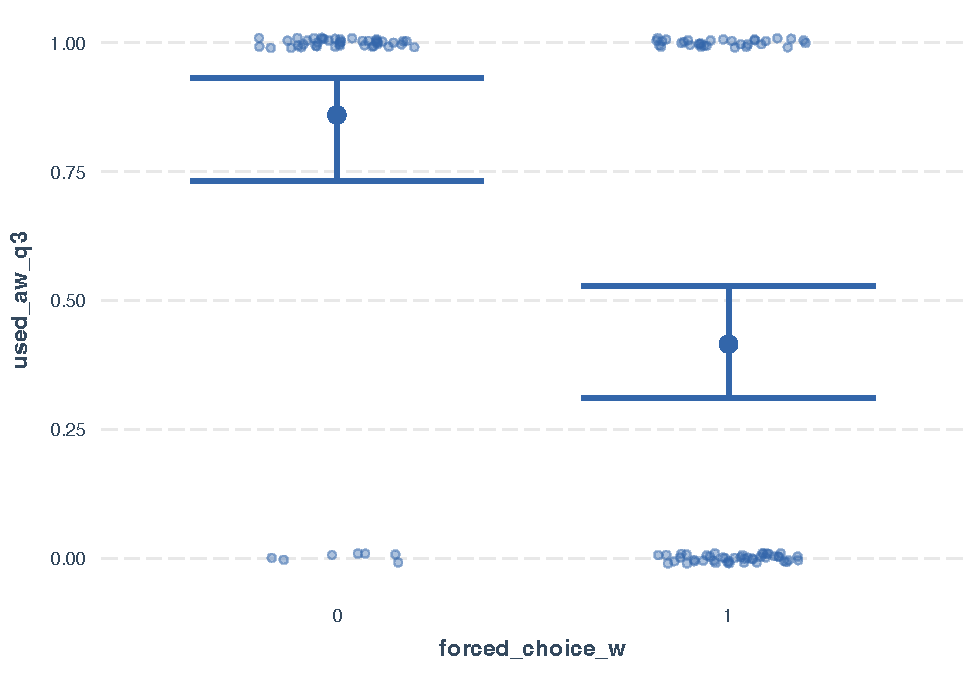
\includegraphics{analysis-July19_files/figure-latex/unnamed-chunk-38-1.pdf}

\begin{Shaded}
\begin{Highlighting}[]
\CommentTok{\# Convert vars for analysis}

\NormalTok{test }\OtherTok{=}\NormalTok{ dfexp2 }\SpecialCharTok{\%\textgreater{}\%} 
  \FunctionTok{mutate}\NormalTok{(}\FunctionTok{across}\NormalTok{(}\FunctionTok{starts\_with}\NormalTok{(}\StringTok{"used"}\NormalTok{), as.numeric)) }

\CommentTok{\#\textquotesingle{} *This worked!!! Saves a lot of time. Mind I should use "across" much more. And apply, lapply, sapply too.*}

\NormalTok{test }\OtherTok{=}\NormalTok{ test }\SpecialCharTok{\%\textgreater{}\%} 
  \FunctionTok{mutate}\NormalTok{(}\AttributeTok{nbing =}\NormalTok{ used\_bing\_q1 }\SpecialCharTok{+}\NormalTok{ used\_bing\_q2 }\SpecialCharTok{+}\NormalTok{ used\_bing\_q3) }\CommentTok{\# This works too!}
\end{Highlighting}
\end{Shaded}

Effect\_plot to show correlations browsers/s.engines controlling for changes in OSX market shares

\end{document}
